%%==================================================
%% chapter03.tex for TJU Master Thesis
%% Encoding: UTF-8
%%==================================================

\chapter{编织层非线性修正理论}


\section{引言}

在上一章中,通过拉伸实验,对软管组件编织层的力学行为进行了研究,得到了不同规格金属纤维编织层拉伸的力位移曲线,也探索出了一套系统的实验方法,简便而准确。本章就立足于实验得到的数据,针对拉伸实验中力位移曲线出现的强烈的非线性,展开研究,并试图给出理论上的解释。


本文第三章中介绍了\ha 编织层的基本理论。同时进行数值仿真的试算,体现了该理论几个不足之处尚待改进:
\begin{compactitem}
	\item 仿真结果仅能符合拉伸力位移曲线的线性部分,非线性段不能吻合;
	\item 该理论不能用于三维有限元分析,只能进行轴对称问题的分析,因为其刚度矩阵缺少切向刚度。
	\item 该理论仅适用于拉伸实验,不能用于内压爆破实验的建模;
	\item 该理论没有提出合适的强度分析方法,不能验证编织层是否发生破坏。
\end{compactitem}

以上几点不足之处,导致该模型被没有广泛使用。拉伸实验一般只是作为软管组件验证力学特性辅助实验手段,而内压荷载是软管组件最为主要的受力状态。


本章首先利用“修正基体”的方法对特征单元的刚度矩阵进行了补充,使其能够满足三维有限元计算的需要。

其次,对\ha 模型编织角理论部分进行了修正,还提出了编织角加速系数$ k $的概念,并对其物理意义进行了讨论。

另外,\ha 模型中“特征单元”并没有考虑编织层中纤维的上下起伏,导致模型偏刚,影响到内压荷载的计算结果。这里对其进行了修正。

拟合拉伸实验的意义在于:明确编织层的本构模型,使得模型能够准确的反应拉伸实验中的力学行为。然后将该模型应用于其他工况的仿真。

\newpage



\section{有限元试算试件}
本章将分析各种因素对编织层非线性行为的影响,将会反复利用有限元模型试算的结果与第四章的实验结果进行对比。为保证各组试算结果间的可比性,每次试算默认取第一次、第二次拉伸实验的两组试件的参数进行试算,其规格参数格如表\ref{tab:characteristics-of-hose-specimen}所示。


\begin{table}[!htb]
	\centering
	\tcaption{试算试件参数}{characteristics of hose specimen}
	\label{tab:characteristics-of-hose-specimen}
	\begin{tabular}{@{\extracolsep{\fill}}>{\hspace{0.5cm}}cccc}
		\toprule
		                 &   试算试件-1    &   试算试件-2    &  \\ \midrule
		实验组别             &   拉伸实验-1    &   拉伸实验-2    &  \\
		试件原标号            &    芯棒-1     &   软管组件-2    &  \\
		软管形式             & 编织层  & 编织层+PTFE内管  &  \\
		编织层外径(mm)        &    7.60     &    7.70     &  \\
		内管内径(mm)         &    /     &    5.01     &  \\
		软管长度(mm)         &    320.0    &    421.5    &  \\
		编织角(\textdegree) &    52.1     &     52.4      &  \\
		股数$\times$根数     & 24$\times$6 & 24$\times$6 &  \\
		钢丝直径(mm)         &     0.2     &     0.2     &  \\
		拉伸量(mm)         &     80     &     160    &  \\
		 \bottomrule
	\end{tabular} 
\end{table}  

\newcommand{\shi}{试算试件-1}
\newcommand{\shii}{试算试件-2}


\section{修正基体理论}

Hachemi的理论将金属纤维简化为2D的特征单元,然后进行平均化得到特征单元的刚度矩阵。事实上这套理论只考虑了纤维本身的力学属性,如\ref{fig:modified-matrix-relation}所示,纤维间关系也是编织层力学特性的重要贡献部分,也是难点所在。

\begin{figure*}[!htb]
\centering
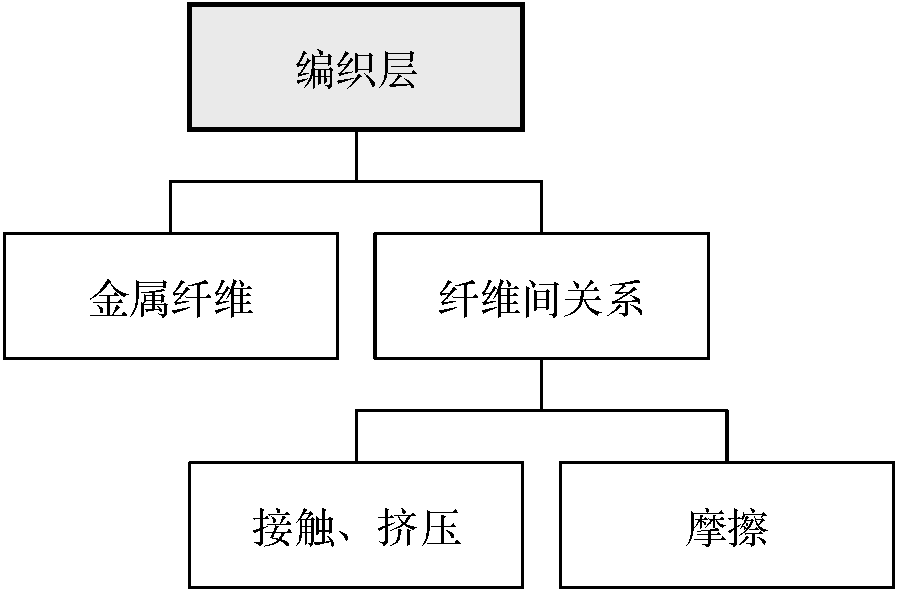
\includegraphics[height=0.2\textheight]{figure/chap5/modified-matrix-relation}
\fcaption{编织层本构关系的内容}{elements of the constitutive relation of braid reinforcement layer}
\label{fig:modified-matrix-relation}
\end{figure*}

编织层纤维简单接触、摩擦往往很难通过理论分析求得。而金属纤维的力学特性相对则是明确的。因此这里引入一种方法:修正基体法(Modified Matrix Method)。

修正基体法最初由\citeauthor{modmm1978}\cite{modmm1978}提出,利用平均化的观点提出来的。修正基体法一般将三维复合材料通过修正的基体模型简化成二维结构,,然后根据现有的理论计算二维编织材料的弹性模量。

尽管有所不同,还是可以利用这种思路,通过基体分担部分纤维的特性,在保留原有纤维理论体系的同时,引入新的纤维间的关系。

实际上编织层是没有基体的。非金属软管加强编织层一般也没有基体。但是纤维间的接触、摩擦对于编织层来说,是独立于纤维的力学特性之外的,起到的作用是稳定、限制结构,类似于基体的作用。那么不妨引入数学上假想的“基体”,对金属纤维本身计算的刚度矩阵进行修正,相当于将金属纤维的接触、摩擦等纤维间关系纳入了“基体”的体系,与纤维本身形成“复合材料”。修正基体可以弥补纤维本身计算的结果与编织层实际力学特性间的差距,起到修正的作用。

参考各向同性材料的刚度矩阵,

\begin{equation}
\label{eq:common-stifness}
\left[ {\begin{array}{*{20}{c}}
{2\mu  + \lambda }&\lambda &\lambda &0&0&0\\
\lambda &{2\mu  + \lambda }&\lambda &0&0&0\\
\lambda &\lambda &{2\mu  + \lambda }&0&0&0\\
0&0&0&\mu &0&0\\
0&0&0&0&\mu &0\\
0&0&0&0&0&\mu 
\end{array}} \right]
\end{equation}

其中, 
\begin{equation}
\mu  = \frac{E}{{2\left( {1 + \nu } \right)}}
\end{equation}

\begin{equation}
\lambda = \frac{{E\nu }}{{\left( {1 + \nu } \right)\left( {1 - 2\nu } \right)}}
\end{equation}


 $ {C_{{\rm{1111}}}} $可以表征两层金属纤维法向接触的刚度(如图 \ref{fig:modifiedmatrix}所示)。将复杂的多点接触的接触刚度简化为各向同性材料内部的弹性刚度,则:

\begin{equation}
{C_{{\rm{1111}}}}{\rm{ = }}\xi E
\end{equation}


$  {C_{{\rm{1212}}}} $、$ {C_{{\rm{1313}}}} $ 对应编织平面内的切向刚度,主要由编织交叠的接触面提供(如图 \ref{fig:modifiedmatrix}所示)。第一次拉伸实验的试件,按照\ha 的基本理论,以\shi 的拉伸量为荷载,进行仿真计算,几次仿真结果赋予不同的$  {C_{{\rm{1212}}}} $、$ {C_{{\rm{1313}}}} $


\begin{figure*}[!htp]
\centering
\subfigure[完整过程]{
	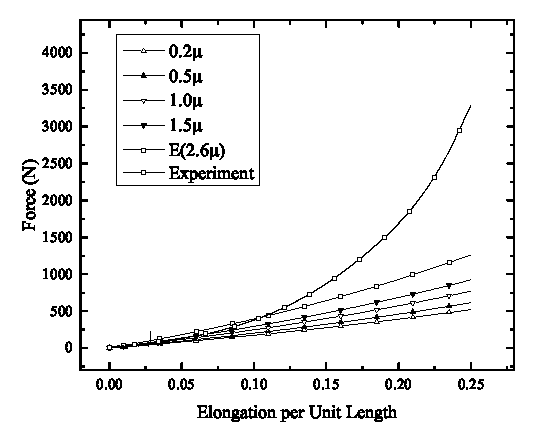
\includegraphics[width=0.45\linewidth]{figure/chap5/Various-Mu.eps}
	\label{fig:VariousMu}
	}
\subfigure[局部(应变$ 0\textasciitilde0.15 $)]{
	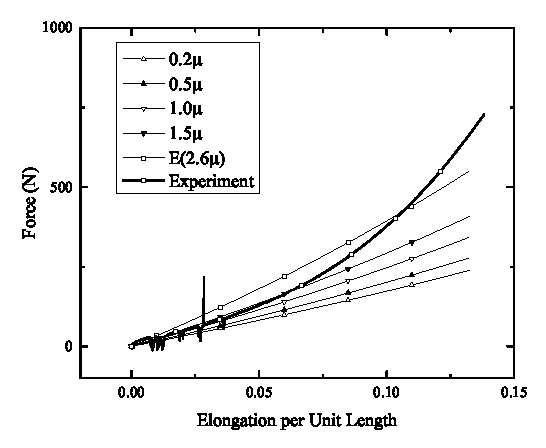
\includegraphics[width=0.45\linewidth]{figure/chap5/Various-Mu-small}
	\label{fig:Various-Mu-small}
	}
\fcaption{不同切向模量模型的力位移曲线}{load displacement  curves of models with various shear moduli}
\end{figure*}




由于编织相当紧密,假设两股纤维正交,单位宽度接触面可以提供相同宽度各向同性材料的切向刚度,根据几何关系,则有:

\begin{figure*}[!htb]
	\centering
	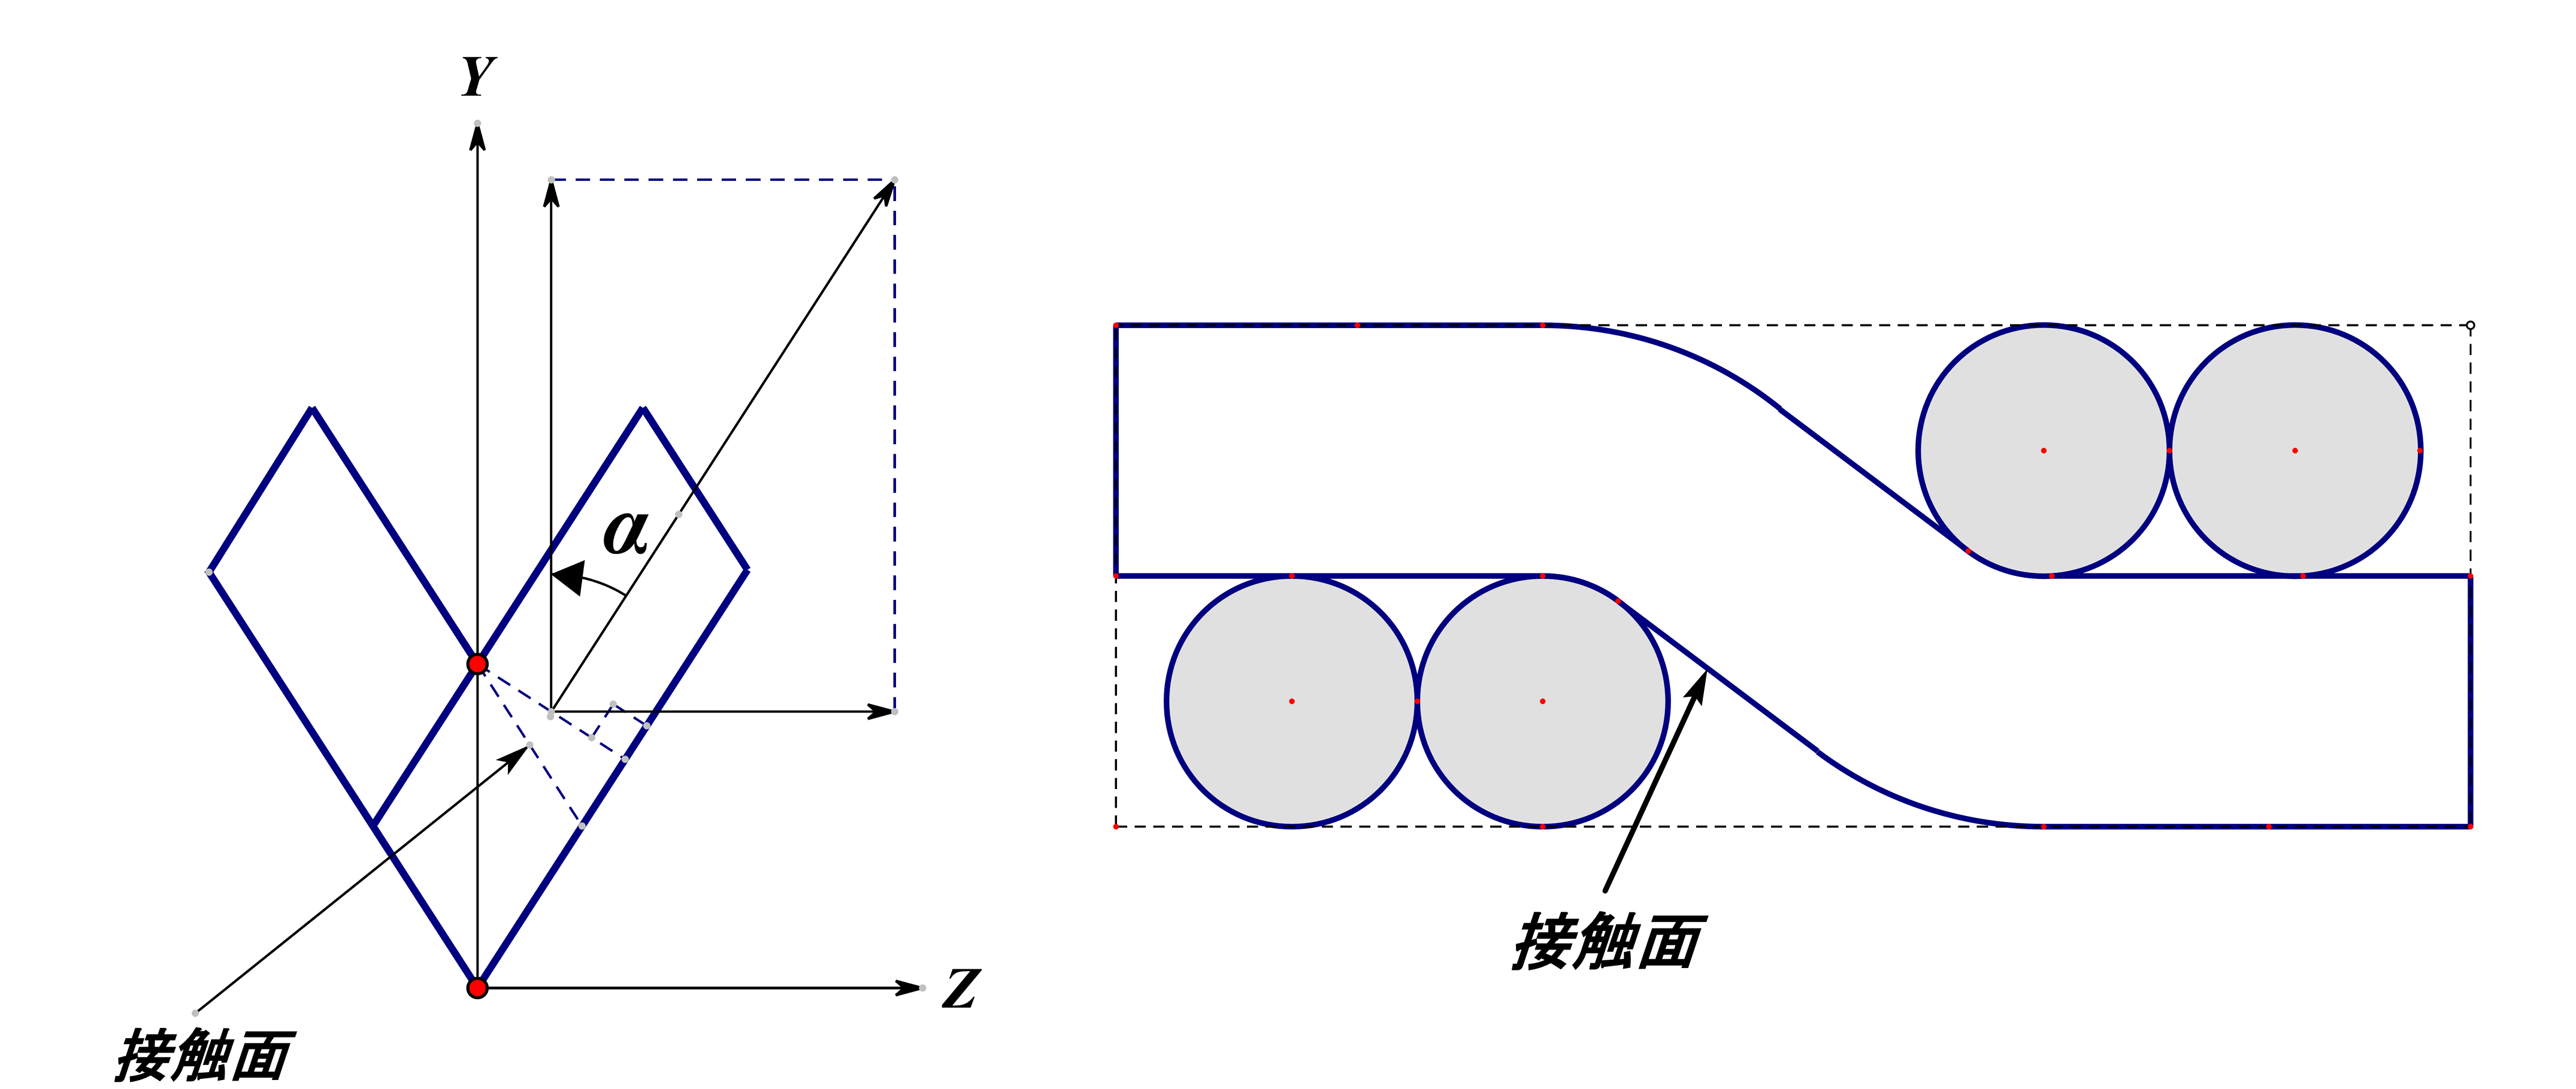
\includegraphics[height=0.25\textheight]{figure/chap5/modified-matrix}
	\fcaption{纤维间接触面几何关系}{geometry of the contact surface between fibers }
	\label{fig:modifiedmatrix}
\end{figure*}

\begin{equation}
\left\{ {\begin{array}{*{20}{c}}
{{C_{1212}} = \xi \mu  \cdot \sin \alpha }\\
{{C_{1313}} = \xi \mu  \cdot \cos \alpha }
\end{array}} \right.
\end{equation}








形成等效修正基体刚度矩阵为:
\begin{equation}
C_{ijkl}^{matrix} = \left[ {\begin{array}{*{20}{c}}
	{E\xi }&0&0&0&0&0\\
	0&0&0&0&0&0\\
	0&0&0&0&0&0\\
	0&0&0&{\mu \xi \cos \alpha }&0&0\\
	0&0&0&0&{\mu \xi \sin \alpha }&0\\
	0&0&0&0&0&0
	\end{array}} \right]
\end{equation}


编织层完整的刚度矩阵为:


\begin{equation}
C_{total}= {C_f} + C_{matrix}
\end{equation}


补充刚度矩阵后,才能进行完整的三维有限元分析。后续的有限计算结构默认补充$ C_{matrix} $。
但是模型仍然不能体现出拉伸试验中的非线性,需要在其他方向继续都模型进行修正。


\subsection{有限元试算结果}

有限元试算结果如\ref{fig:shisuan-1}所示。结合修正基体法后,基本没有表现出非线性行为。但从有限元仿真的角度来说,这是一个必要的过程,因为要进行更贴近实际工况的仿真,必须采用三维单元。补充修正刚度之后,刚度矩阵才满足$ 6\times6 $,可以进行三维有限元分析。
\begin{figure*}[!htp]
\centering
\subfigure{
	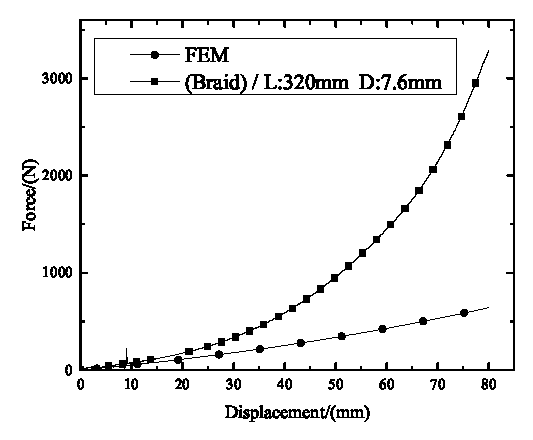
\includegraphics[width=0.45\linewidth]{figure/chap5/Ex-1-Origin}
	\label{fig:Ex-1-Origin}
	}
\subfigure{
	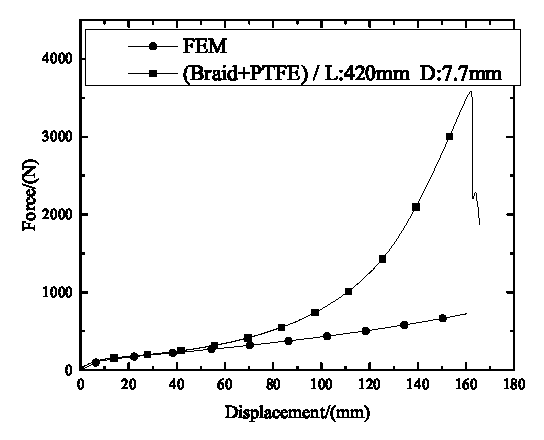
\includegraphics[width=0.45\linewidth]{figure/chap5/Ex-2-Origin}
	\label{fig:Ex-2-Origin}
	}
\fcaption{经过"修正基体法"修正的模型力位移曲线}{load displacement curve of the models modified by "modified matrix method"}
\label{fig:shisuan-1}
\end{figure*}



\section{编织角加速系数}


对比有限元模型与实验测得的编织角的变化,实验中编织角变化的速度更快(如图 \ref{fig:Graph30}所示),因此需要修正编织角理论,加速编织角的变化。
 
 \begin{figure*}[!htp]
\centering
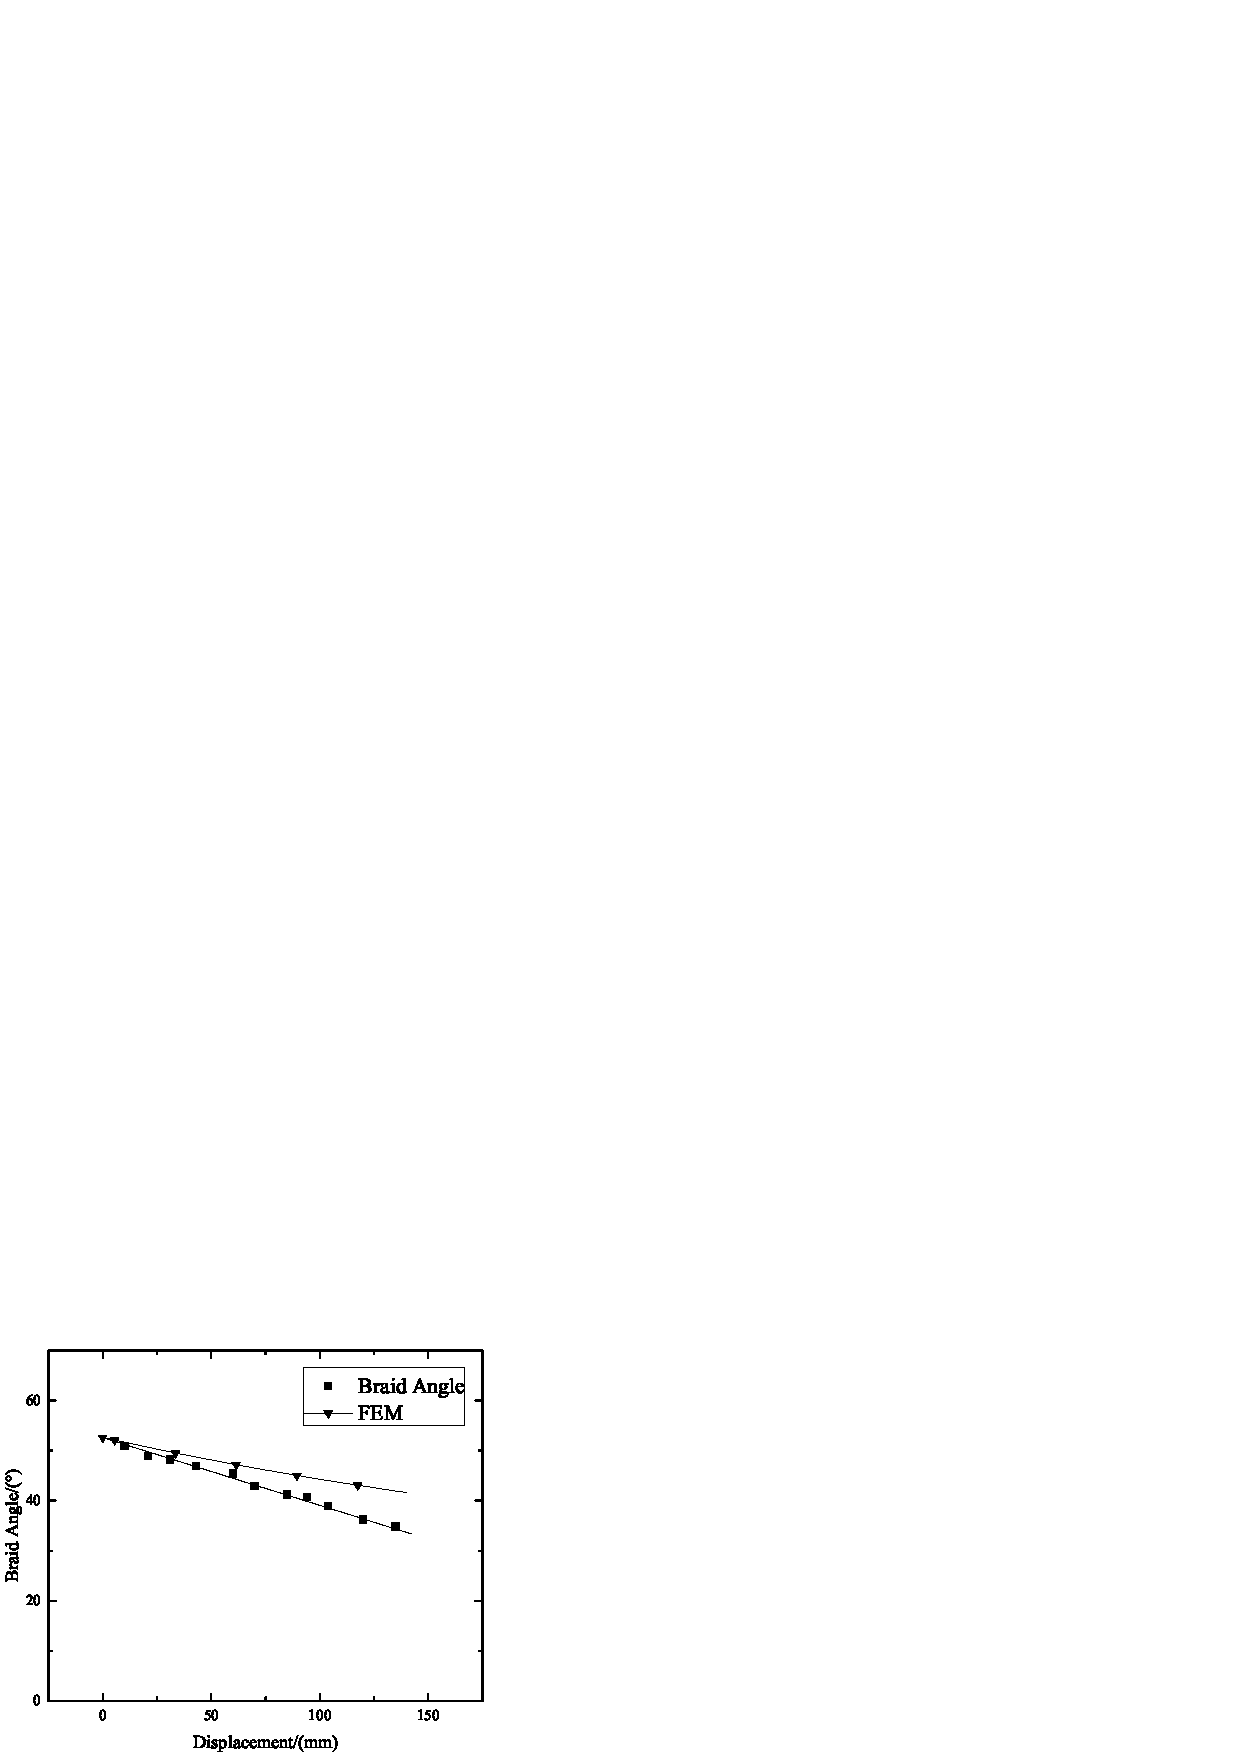
\includegraphics[width=0.5\linewidth]{figure/chap5/Graph30}
\fcaption{编织角变化实验结果对比有限元仿真结果(编织角-位移曲线)}{contrast of experimental and FEM results in braid angle change}[有限元编织角变化对比]
\label{fig:Graph30}
\end{figure*}

这种接触没有包含在等效修正基体中。金属纤维发生角度变化的过程中,各股金属纤维之间的侧向接触关系较为复杂,同时偶合了纤维本身的弯曲、扭转、摩擦等复杂情况。
这里提出一个简化假设:假设这些复杂的传力机制在编织层轴向上产生的效果,假设可以简化为特征单元轴向上的一组性弹簧,如图 \ref{fig:k-2}。 $ \alpha $ 可以该理解为特征单元中传力路径的方向,可以通过使得特征单元受力平衡的外力的偏离轴向的角度来表征。由于轴向弹簧、金属纤维的伸长,最终会合成一个偏离金属纤维的合力,则如图\ref{fig:k-3}所示,特征单元平衡时外力将会有 的额外转角。
\begin{figure*}[!htp]
\centering
	\hspace{0.5cm}
\subfigure[]{
	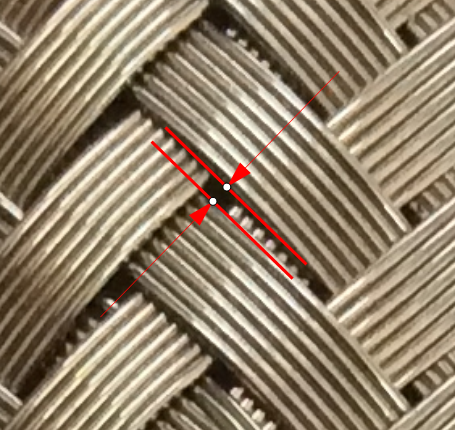
\includegraphics[height=0.12\textheight]{figure/chap5/k/1}
	\label{fig:k-1}
	}
	\hspace{0.5cm}
\subfigure[]{
	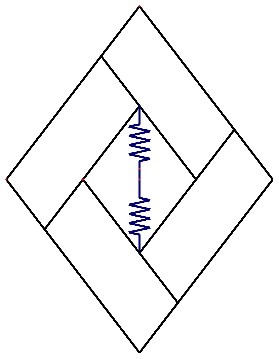
\includegraphics[height=0.13\textheight]{figure/chap5/k/2}
	\label{fig:k-2}
}
	\hspace{0.5cm}
\subfigure[]{
	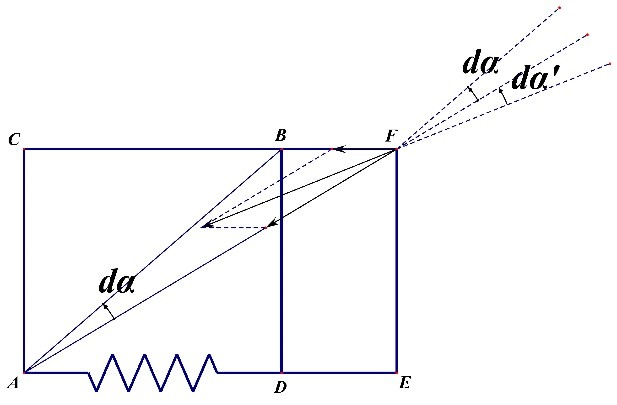
\includegraphics[height=0.15\textheight]{figure/chap5/k/3}
	\label{fig:k-3}
}
\fcaption{加速系数的模型}{model of braid angle coefficient }
\end{figure*}



这就需要编织角理论能够反映这种额外的转角。在(8)式中引入加速编织角变化的经验修正函数 $ \Phi \left( {\alpha ,D} \right) $,$ \alpha  $ 、$ D $ 分别为编织角与直径,表示该函数可能与软管的几何参数相关。
	  
	  

\begin{equation}
d\alpha  = \Phi \left( {\alpha ,D} \right) \cdot \frac{{{\varepsilon _{22}}\sin \alpha \cos \alpha }}{{1 + {\varepsilon _{22}}{{\cos }^2}\alpha }}
\end{equation}


根据实验结果及提出的假设:编织角变化在加载速度恒定的位移荷载下呈线性变化。因此,经验修正函数可能仅包含常数项:


\begin{equation}
\Phi \left( {\alpha , D} \right) = k
\end{equation}


\subsection{有限元试算结果}

$ k $ 值由不同的编织结构确定。按照修正编织角理论,有限元计算结果如图 \ref{fig:k-results}所示: 

\begin{figure*}[!htp]
\centering
\subfigure[$ k=3.0 $( 试算试件-1)]{
	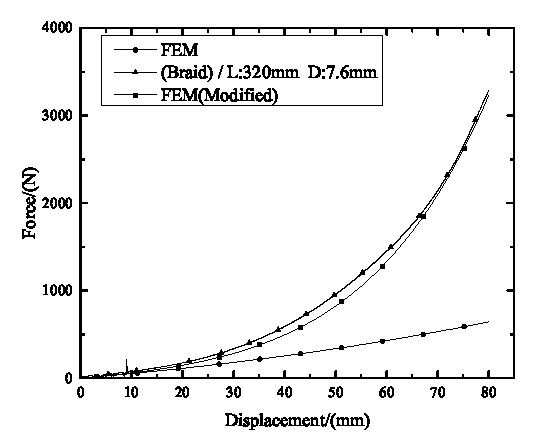
\includegraphics[height=0.2\textheight]{figure/chap5/Ex-1-Com}
	\label{fig:k-Ex-1-Com}
	}
\subfigure[$ k=2.3 $ ( 试算试件-2)]{
	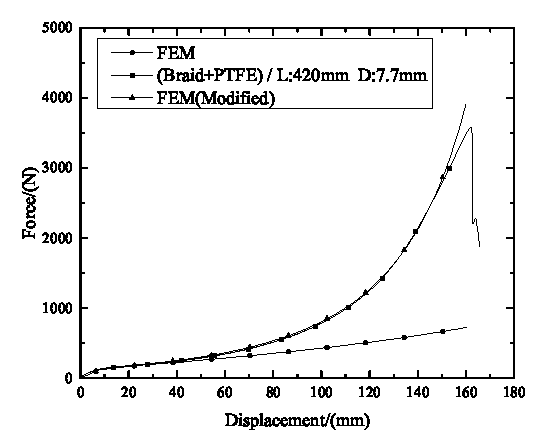
\includegraphics[height=0.2\textheight]{figure/chap5/Ex-2-Com}
	\label{fig:k-Ex-2-Com}
}
\subfigure[实验3-1-BD90]{
	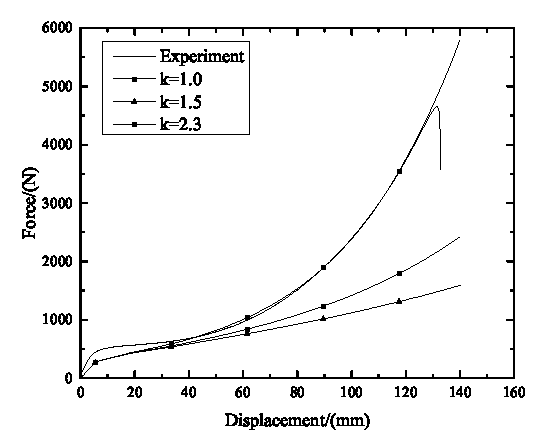
\includegraphics[height=0.2\textheight]{figure/chap5/Graph29}
	\label{fig:k-Graph28}
}
\subfigure[有限元编织角变化与实验对比]{
	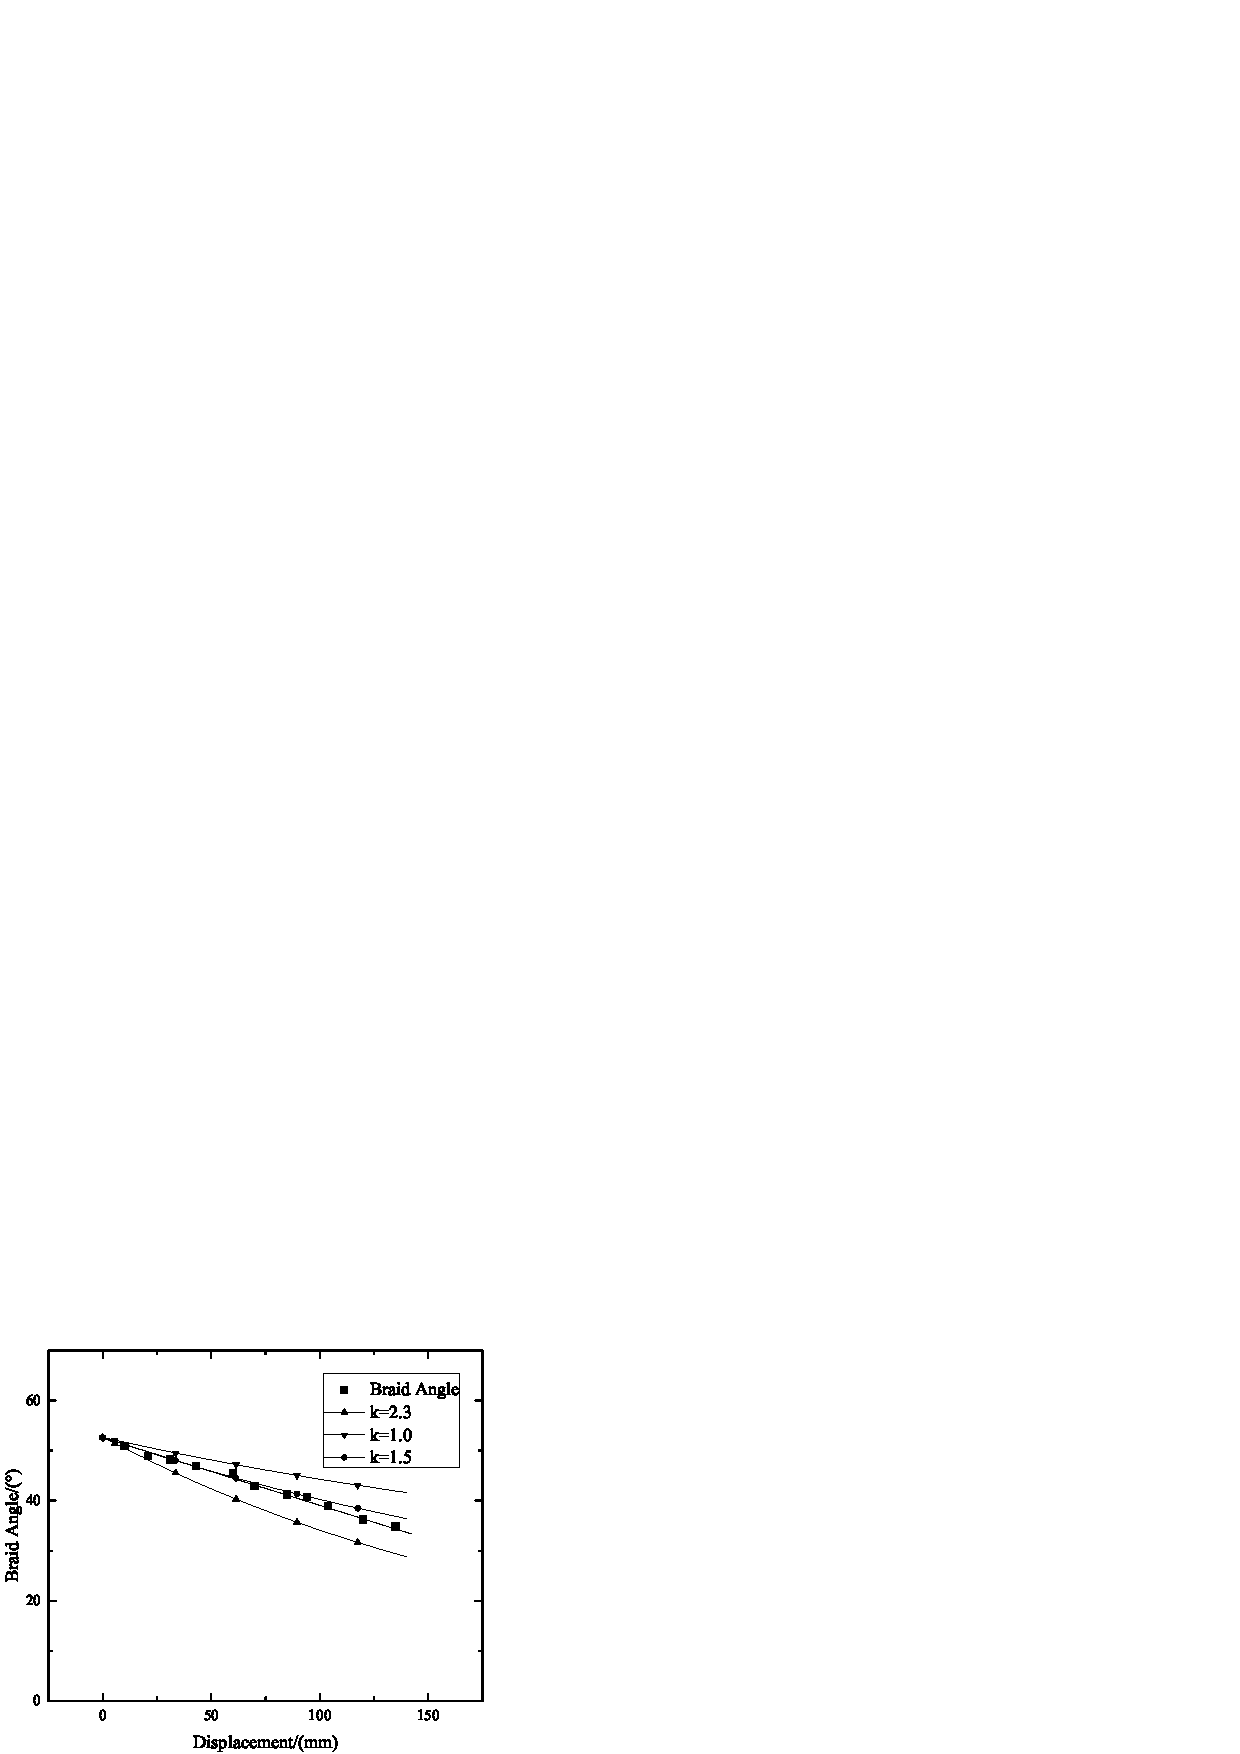
\includegraphics[height=0.2\textheight]{figure/chap5/Graph28}
	\label{fig:k-Graph29}
}
\fcaption{加速系数$ k $修正后的有限元仿真结果}{FEM results of models modifed by braid angle coefficient }
\label{fig:k-results}
\end{figure*}






图 \ref{fig:k-Graph28}、\ref{fig:k-Graph29}中,分别为$ k $取不同值时,软管模型力-位移曲线、编织角变化曲线。可以发现,当
$ k=2.3 $时,有限元模型的力-位移曲线与实验基本吻合,但编织角的变化的趋势要大于实验;当$ k=1.5 $时,有限元模型的编织角变化趋势与实验相近,但力-位移曲线趋势与实验相差较大。这意味着当编织角确定时,修正后的单元刚度仍小于实际情况;也可以认为,本模型可以表征金属编织软管的拉伸受力情况,但编织角偏转的理论值要大于实际值,有限元模拟中$ \alpha $ 超过实际编织角的部分就是由这部分额外的转角导致的。因此,加速系数k实际上有着很大的物理意义,它实际上涵盖了金属纤维间侧向接触,以及纤维间摩擦的作用效果。


尽管这种接触可以等效为弹簧,但是确定弹簧的弹性系数比较困难,因为这个系数很有可能是非线性的:单股纤维转动时,首先填满各股之间空隙,此时轴向弹性较小;随着拉伸荷载增大,纤维自身弯曲扭转,纤维间压紧,摩擦增大,轴向弹性效果可能会明显增强。要量化确定这个过程,需要进一步实验的支持。

另外,尽管编织角加速系数能够取得较好的拟合拉伸实验的效果,但是该方法“覆盖”了其他因素。因此,本研究还要对影响编织层刚度的因素进行进一步的分析,将编织角加速系数作为最终补充的拟合手段。


\section{编织角理论修正}
\ha 的理论中,编织层管径的变化采用钢绞线理论,如式\ref{eq:d-chap5}所示。但是这样的处理方法并不能准确的反应管径的变化,从结果上来时导致了整体非线性不足

\begin{equation}
\label{eq:d-chap5}
D = {D_0}\frac{{\sin \left( \alpha  \right)}}{{\sin \left( {{\alpha _0}} \right)}},
L = {L_0}\frac{{\cos \left( \alpha  \right)}}{{\cos \left( {{\alpha _0}} \right)}}
\end{equation}



而软管组件的内管刚度较低容易被压缩;受内压荷载的状态下,管径的变化也是一个很重要的因素,因此管径的变化应该直接在特征单元中体现。图\ref{fig:unit-cell-3}为特征单元考虑管径的修正方案。根据几何关系可得:

\begin{figure*}[!htb]
\centering
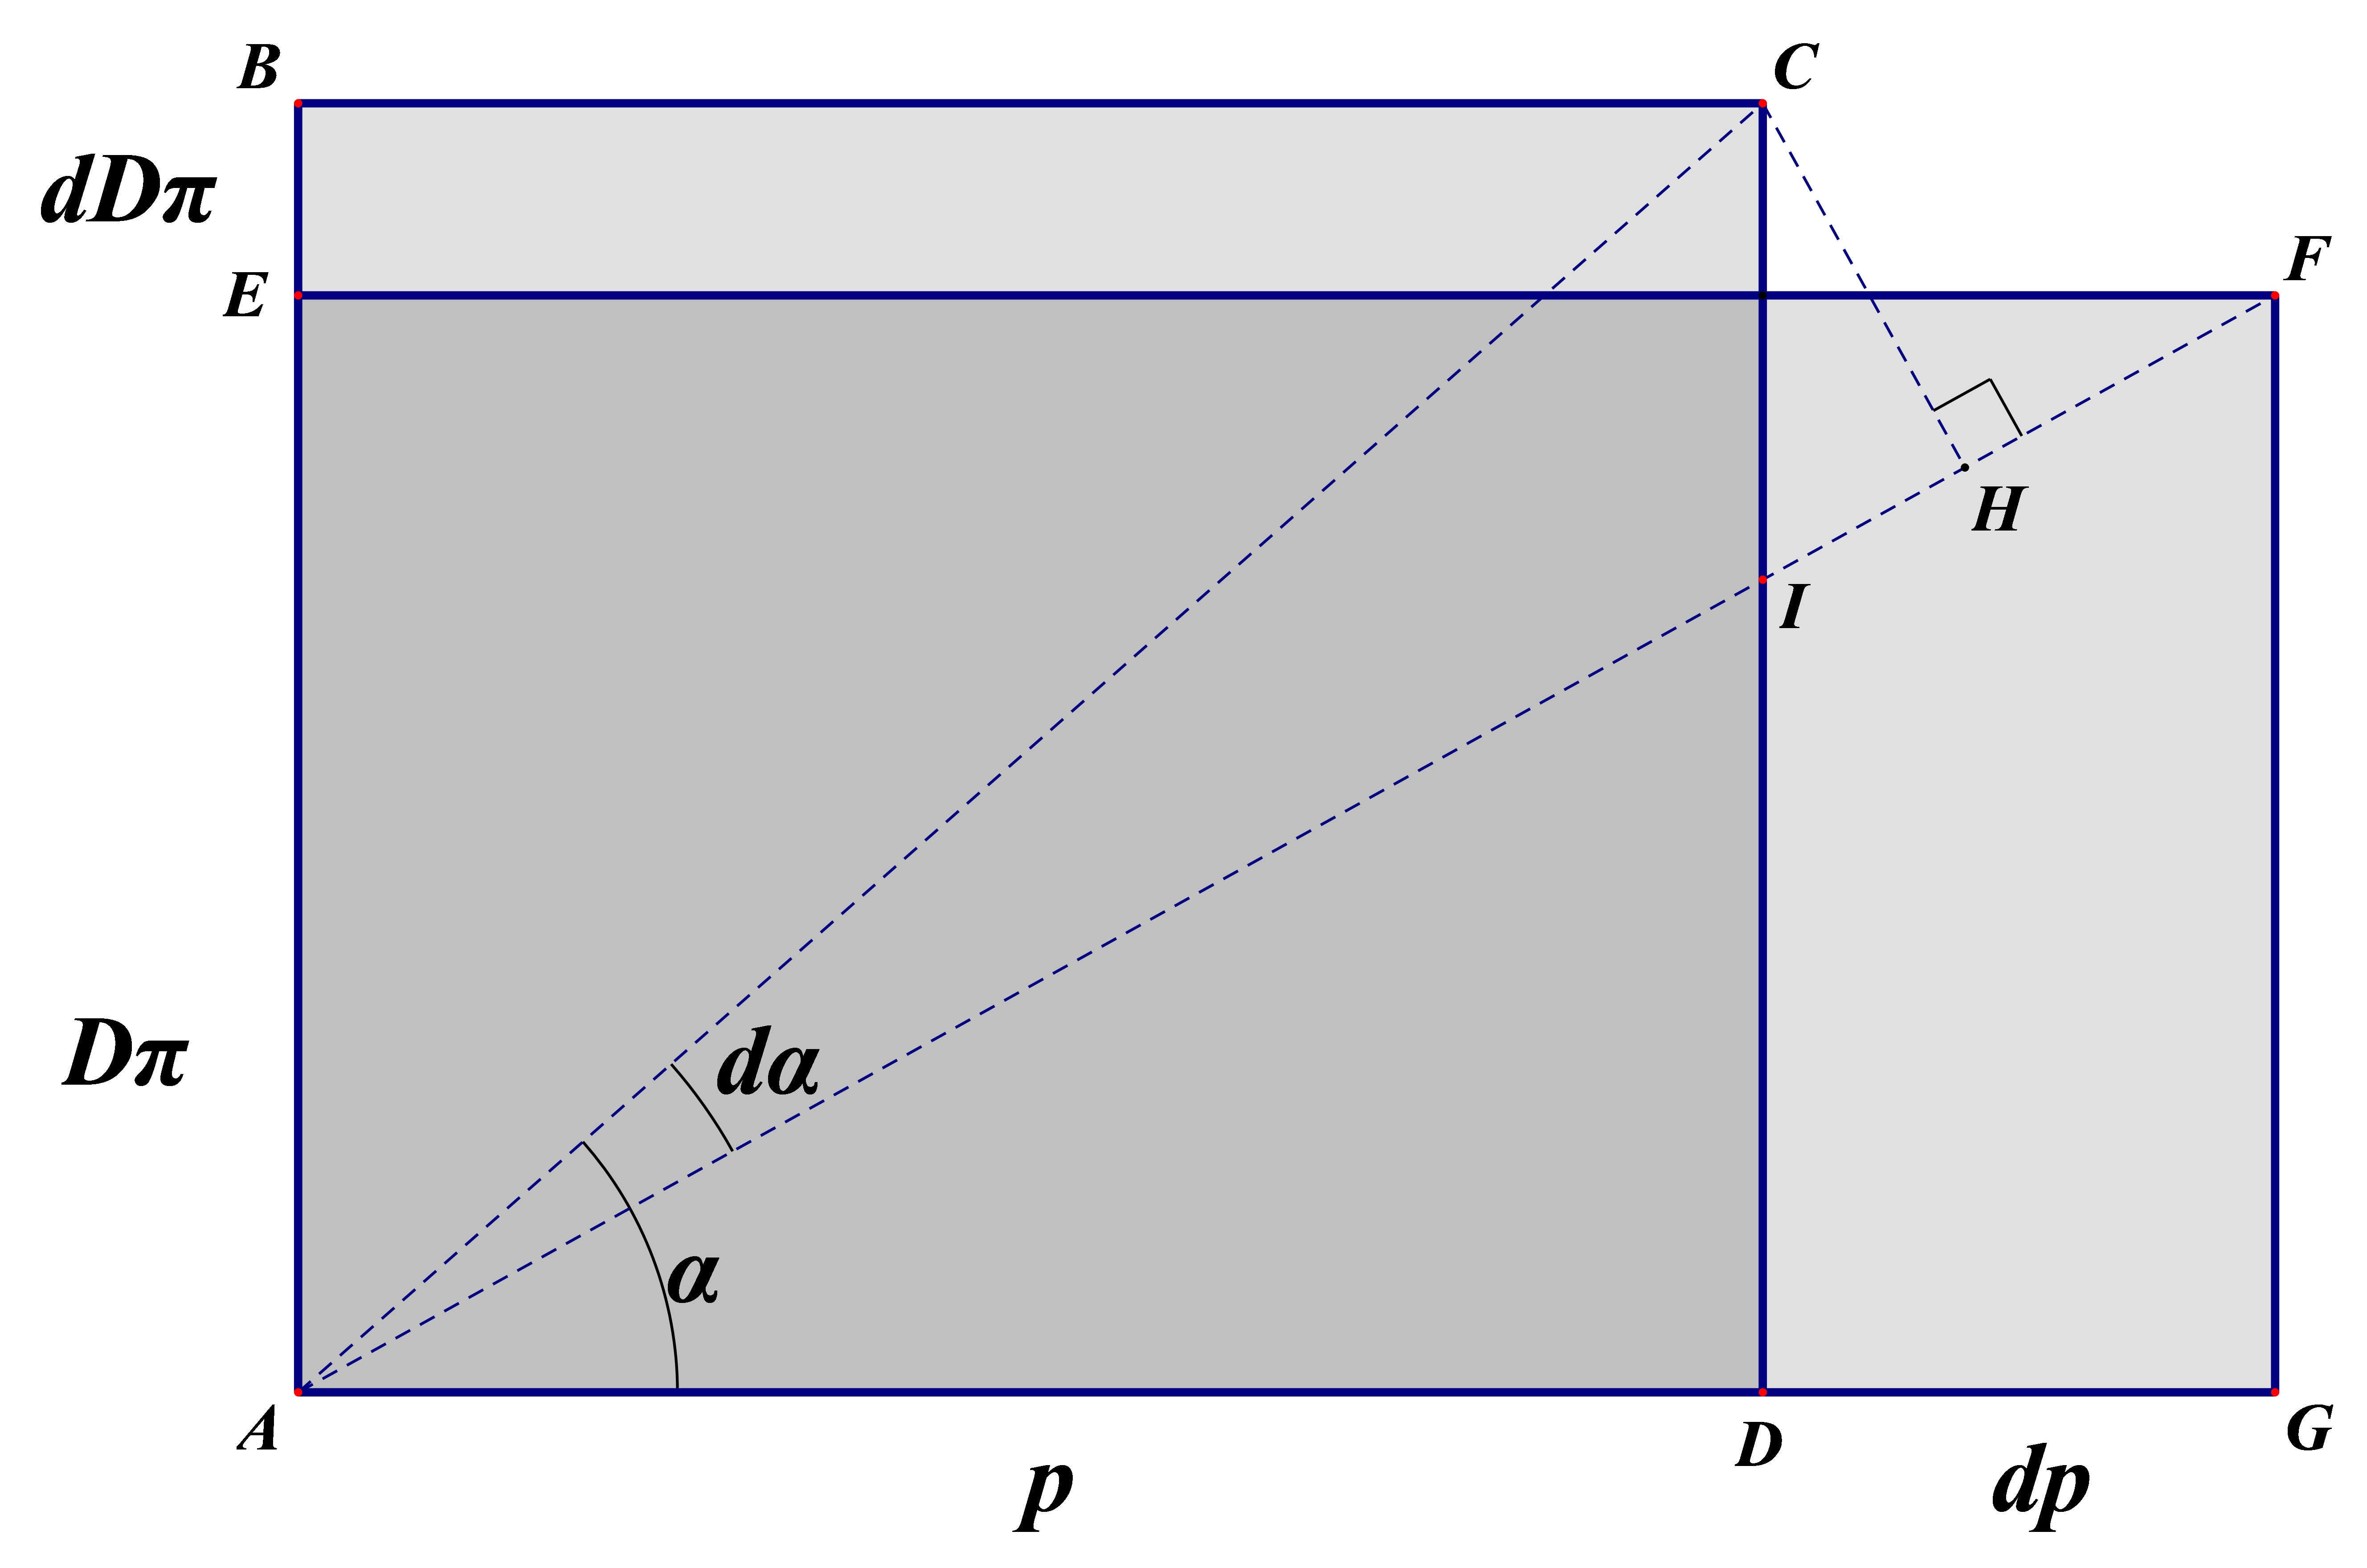
\includegraphics[height=0.2\textheight]{figure/chap5/unit-cell-3}
\fcaption{特征单元的编织角变化几何关系修正}{modified geometry of braid angle change}
\label{fig:unit-cell-3}
\end{figure*}

纤维的伸长量为:

\begin{equation}
\begin{array}{*{20}{c}}
{{\varepsilon _{33}} = \frac{{dD}}{D}}&{{\varepsilon _{22}} = \frac{{dP}}{P}}
\end{array}
\end{equation}

\begin{equation}
d\alpha  = \frac{{\left( {{\varepsilon _{22}} + {\varepsilon _{33}}} \right)\sin \left( \alpha  \right){\rm{cos}}\left( \alpha  \right)}}{{1 - {\varepsilon _{33}}{{\sin }^2}\left( \alpha  \right) + {\varepsilon _{22}}{\rm{co}}{{\rm{s}}^2}\left( \alpha  \right)}}
\end{equation}


\begin{equation}
{\varepsilon _f} = \sqrt {\frac{{{{\left( {{\varepsilon _{22}} + 1} \right)}^2} + \tan {\alpha ^2}{{\left( {1 - {\varepsilon _{33}}} \right)}^2}}}{{1 + \tan {\alpha ^2}}}}  - 1
\end{equation}


\subsection{有限元试算结果}
利用修正后的编织角理论进行有限元仿真试算,结果如图\ref{fig:RUC-MOD}所示,力位移曲线出现了明显的非线性。
\begin{figure*}[!htp]
\centering
\subfigure[实验试件-1]{
	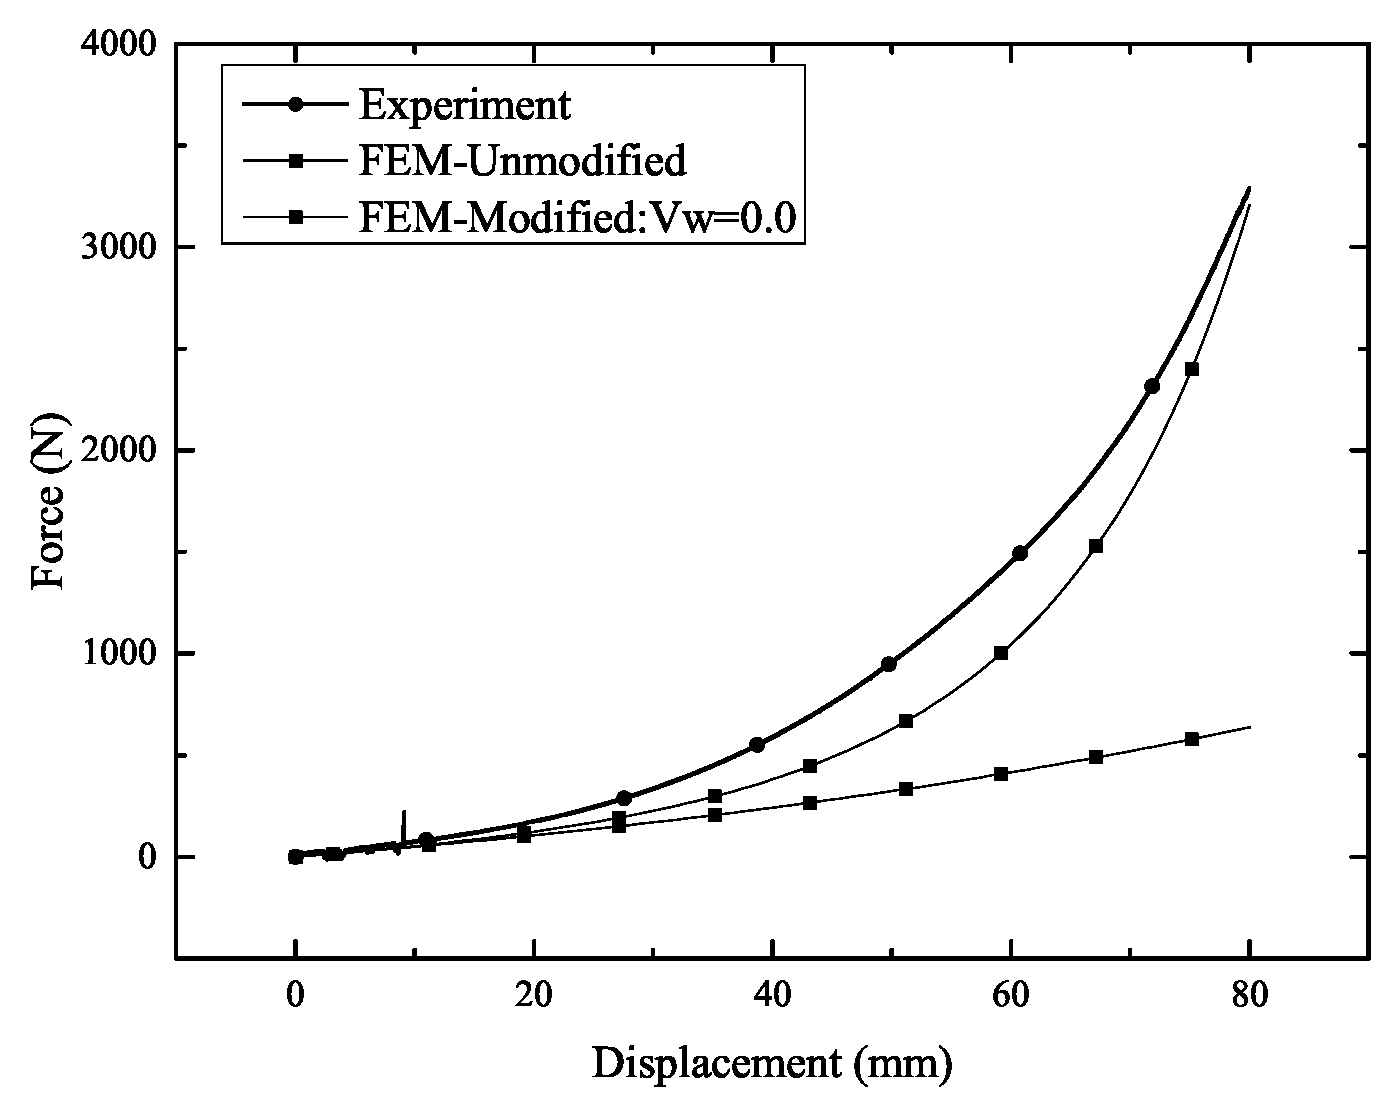
\includegraphics[width=0.45\linewidth]{figure/chap5/sp1/RUC-mod}
	}
\subfigure[实验试件-2]{
	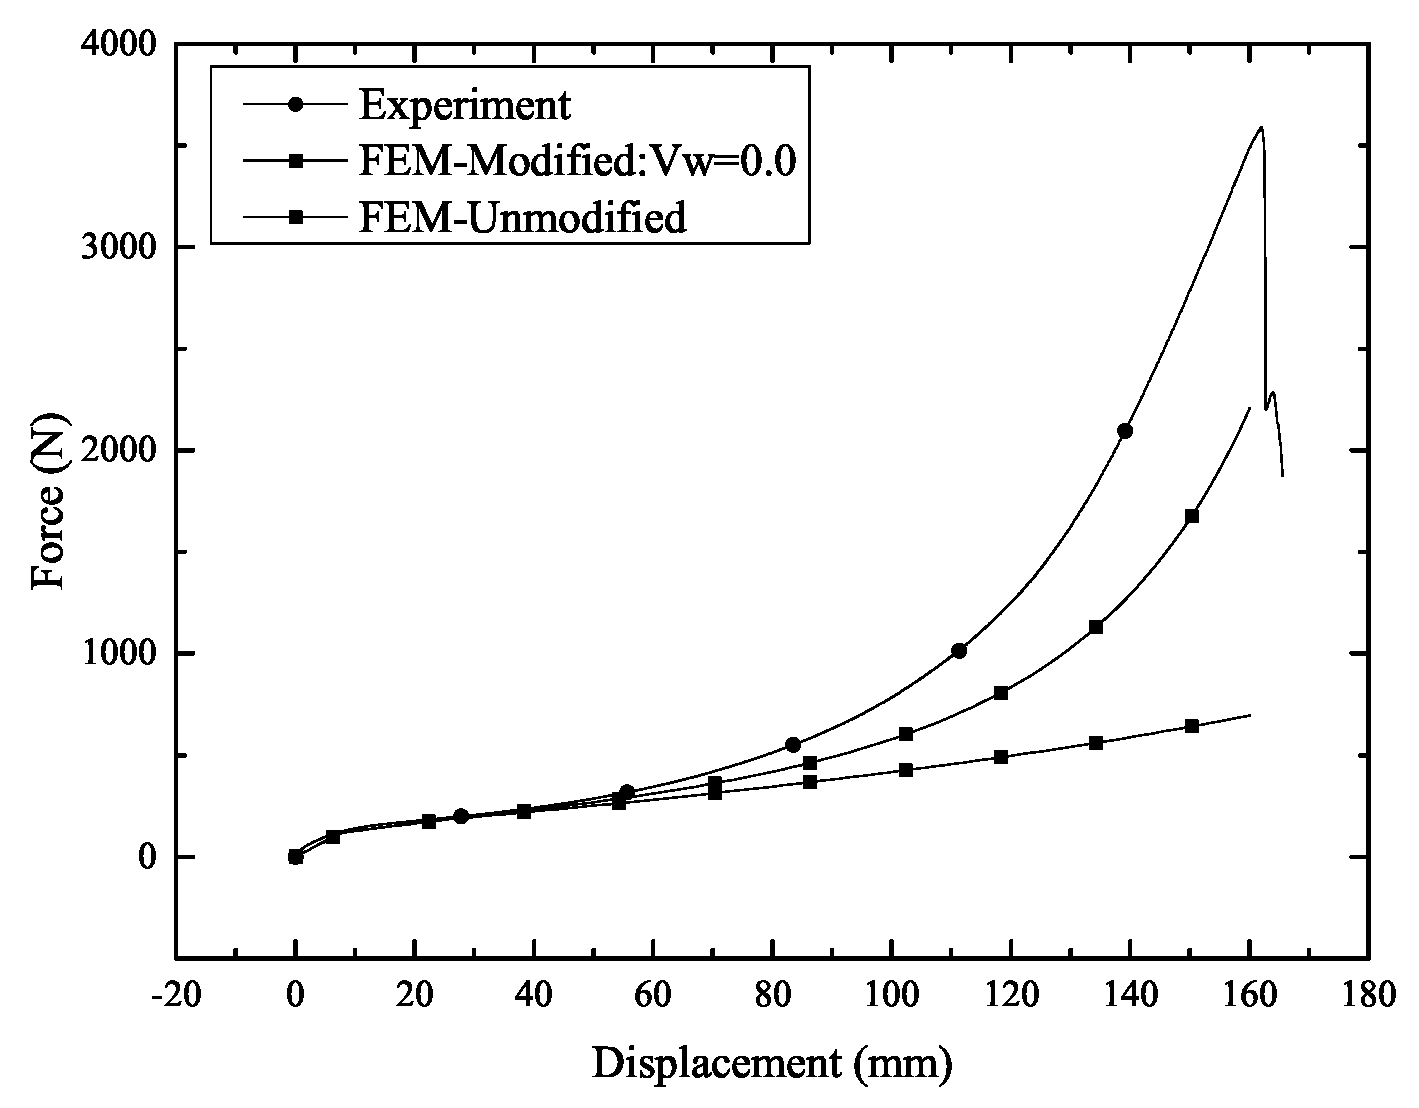
\includegraphics[width=0.45\linewidth]{figure/chap5/sp2/RUC-MOD}
	}
\fcaption{修正编织角理论有限元试算结果}{FEM Results of Models with Modified Braided Angel}
\label{fig:RUC-MOD}
\end{figure*}






\section{三维线型修正}

实际上,仅仅把纤维简化为平面2D的特征单元是不够的,实际如\ref{fig:3d-wire-3}所示,对于$ 2\times 2 $编织形式的非金属纤维编织层,至少$ 50 \% $的纤维处于斜穿状态。

\subsection{斜穿纤维角度的计算}
一般高密度编织层中,纤维相互紧贴,截面编织密度$ {\xi _{section}} \approx 1 $,根据式\ref{eq:section-epsilon}可得编织层厚度,也就是斜穿纤维厚度方向上传过的距离为:


\begin{equation}
\tau \phi  = D - \sqrt {{D^2} - \frac{{{N_S}{N_W}{\phi ^2}}}{{\cos \alpha }}} 
\end{equation}

如图\ref{fig:3d-wire-3}所示,斜穿的纤维,投影在编织平面内的头投影的长度为:
\begin{equation}
\frac{{{N_W}\phi }}{{\sin 2\alpha }}
\end{equation}
则斜穿纤维偏离平面的角度为
\begin{equation}
\frac{\pi }{2} - \varphi  = \arctan \frac{{\tau \phi}}{{{N_W}\phi }}
\end{equation}

以\shii 为例,将其参数代入可得纤维偏离平面的角度$ \frac{\pi }{2} - \varphi  $为$ 26.9\textdegree $。



\subsection{考虑斜穿纤维的刚度计算}

对于金属纤维的编织层,金属纤维由于刚度较高,会保持类似于正弦函数图像的线型。如图\ref{fig:sin-xianxing}所示。这也导致了一层金属编织层的厚度一般大于两层缠绕成。针对这种弯曲纤维,\citeauthor{russia1970}\cite{russia1970}提出了一种处理方法:

\begin{figure*}[!htb]
\centering
\subfigure[]{
	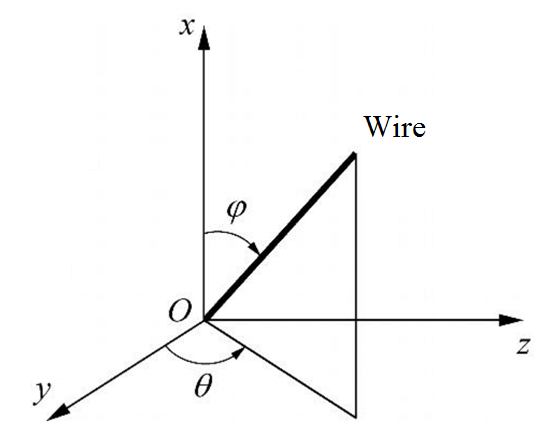
\includegraphics[height=0.2\textheight]{figure/chap5/3d-wire}
	}
\hspace{0.5cm}
\subfigure[]{
	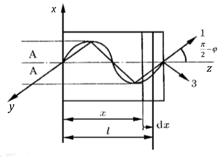
\includegraphics[height=0.2\textheight]{figure/chap5/3d-wire-2}
	\label{fig:sin-xianxing}
	}
\fcaption{编织层中斜穿的纤维}{Interlacing fiber in the Braid Layer}
\label{fig:3d-wire}
\end{figure*}






假设图	\ref{fig:sin-xianxing}中的纤维轨迹服从函数 $  f\left( x \right)$ 的规律,与平面的夹角$ \theta $可表示成:

\begin{equation}
\frac{\pi }{2} - \varphi   =  - \arccos \frac{1}{{\sqrt {1 + {{\left( {A\frac{{df\left( x \right)}}{{dx}}} \right)}^2}} }}
\end{equation}

结合修正基体法根据单向纤维复合材料微段$ dx $的柔度系数$ {{S_{ij}}^*\left( \frac{\pi }{2} - \varphi  \right)} $,通过曲线积分求得相应编织材料的有效性能为:

\begin{equation}
{S_{ij}} = \frac{1}{l}\int\limits_0^l {{S_{ij}}^*\left( \frac{\pi }{2} - \varphi \right)dx} 
\end{equation}

但这种处理方相对较为繁琐,本文选择较为类似的一种处理方法。$ 2\times 2 $编织形式可以近似看作图\ref{fig:3d-wire-3}中的形式,将编织层分为间隔交替的两种纤维分布形式。


\begin{figure*}[!htp]
	\centering
	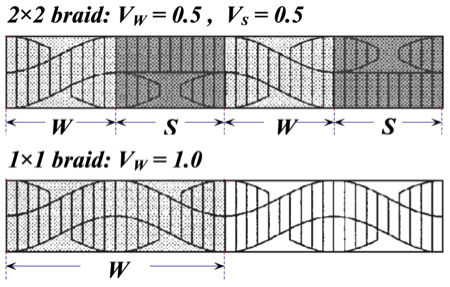
\includegraphics[height=0.2\textheight]{figure/chap5/3d-wire-3}
	\label{fig:3d-wire-3}
	\fcaption{不同编织形式中斜穿纤维的分布}{distribution of interlacing fiber in the braid layer}
\end{figure*}

其中$ V_W $为斜穿纤维的体积比例;$ V_S $为平面内纤维的体积比例,纤维编织层整体的刚度矩阵为

\begin{equation}
{C_f} = {V_S} \cdot {C_{f,ijkl}}^S + {V_W} \cdot {C_{f,ijkl}}^W
\end{equation}

其中,$ {C_{f,ijkl}}^S $为平面内钢丝的刚度矩阵;为斜穿纤维部分的刚度矩阵,需要额外考虑纤维的取向,如图\ref{fig:3d-wire}所示,则有:

\begin{equation}
\left\{ \begin{array}{l}
{n_1} = \cos \varphi \\
{n_2} = sin\varphi \sin \theta \\
{n_3} = sin\varphi \cos \theta 
\end{array} \right.
\end{equation}

那么斜穿部分纤维的刚度矩阵$ {C_{f,ijkl}}^W $为:

\begin{equation}\small
E\xi  \cdot \left[ {\tiny \begin{array}{*{20}{c}}
{{{\cos }^4}\varphi }&{{{\cos }^2}\varphi {{\cos }^2}\theta }&{{{\cos }^2}\varphi {{\sin }^2}\theta }&{{{\cos }^3}\varphi \cos \theta }&0&0\\
{{{\cos }^2}\varphi {{\cos }^2}}&{{{\cos }^4}\theta }&{{{\cos }^2}\theta {{\sin }^2}\theta }&{\cos \varphi {{\cos }^3}\theta }&0&0\\
{{{\cos }^2}\varphi {{\sin }^2}\theta }&{{{\cos }^2}\theta {{\sin }^2}\theta }&{{{\sin }^4}\theta }&{\cos \varphi \cos \theta {{\sin }^2}\theta }&0&0\\
{{{\cos }^3}\varphi \cos \theta }&{\cos \varphi {{\cos }^3}\theta }&{\cos \varphi \cos \theta {{\sin }^2}\theta }&{{{\cos }^2}\varphi {{\cos }^2}\theta }&0&0\\
0&0&0&0&{{{\cos }^2}\varphi {{\sin }^2}\theta }&{\cos \varphi \cos \theta {{\sin }^2}\theta }\\
0&0&0&0&{\cos \varphi \cos \theta {{\sin }^2}\theta }&{{{\cos }^2}\theta {{\sin }^2}\theta }
\end{array}} \right]
\end{equation}

\subsection{斜穿纤维角度的影响}

斜穿纤维偏离编织层平面的角度为$ \frac{\pi }{2} - \varphi  $,图\ref{fig:phi-MOD}中分别为$ \frac{\pi }{2} - \varphi  = 0\textdegree/20\textdegree/40\textdegree/60\textdegree$的力位移曲线。该角度减小时,编织层整体在拉伸的过程中会体现更强的非线性,整体的刚度也会加强。
\begin{figure*}[!htp]
	\centering
	\subfigure[试验试件-1]{
		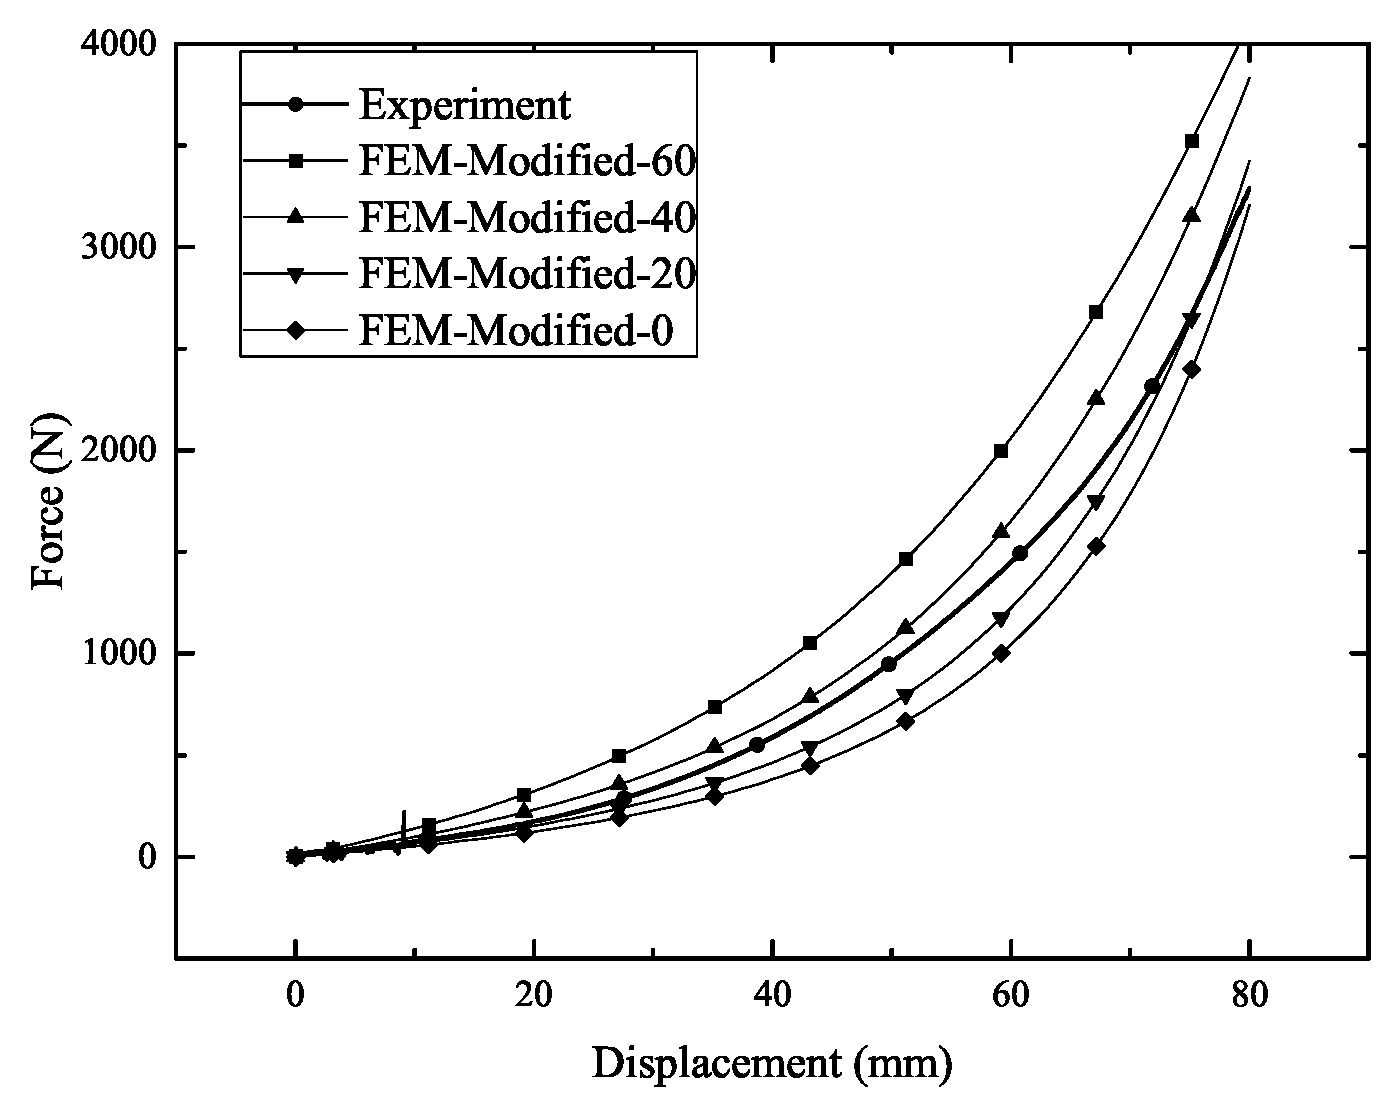
\includegraphics[height=0.35\textheight]{figure/chap5/sp1/phi-mod}
		}
		
	\subfigure[试验试件-2]{
		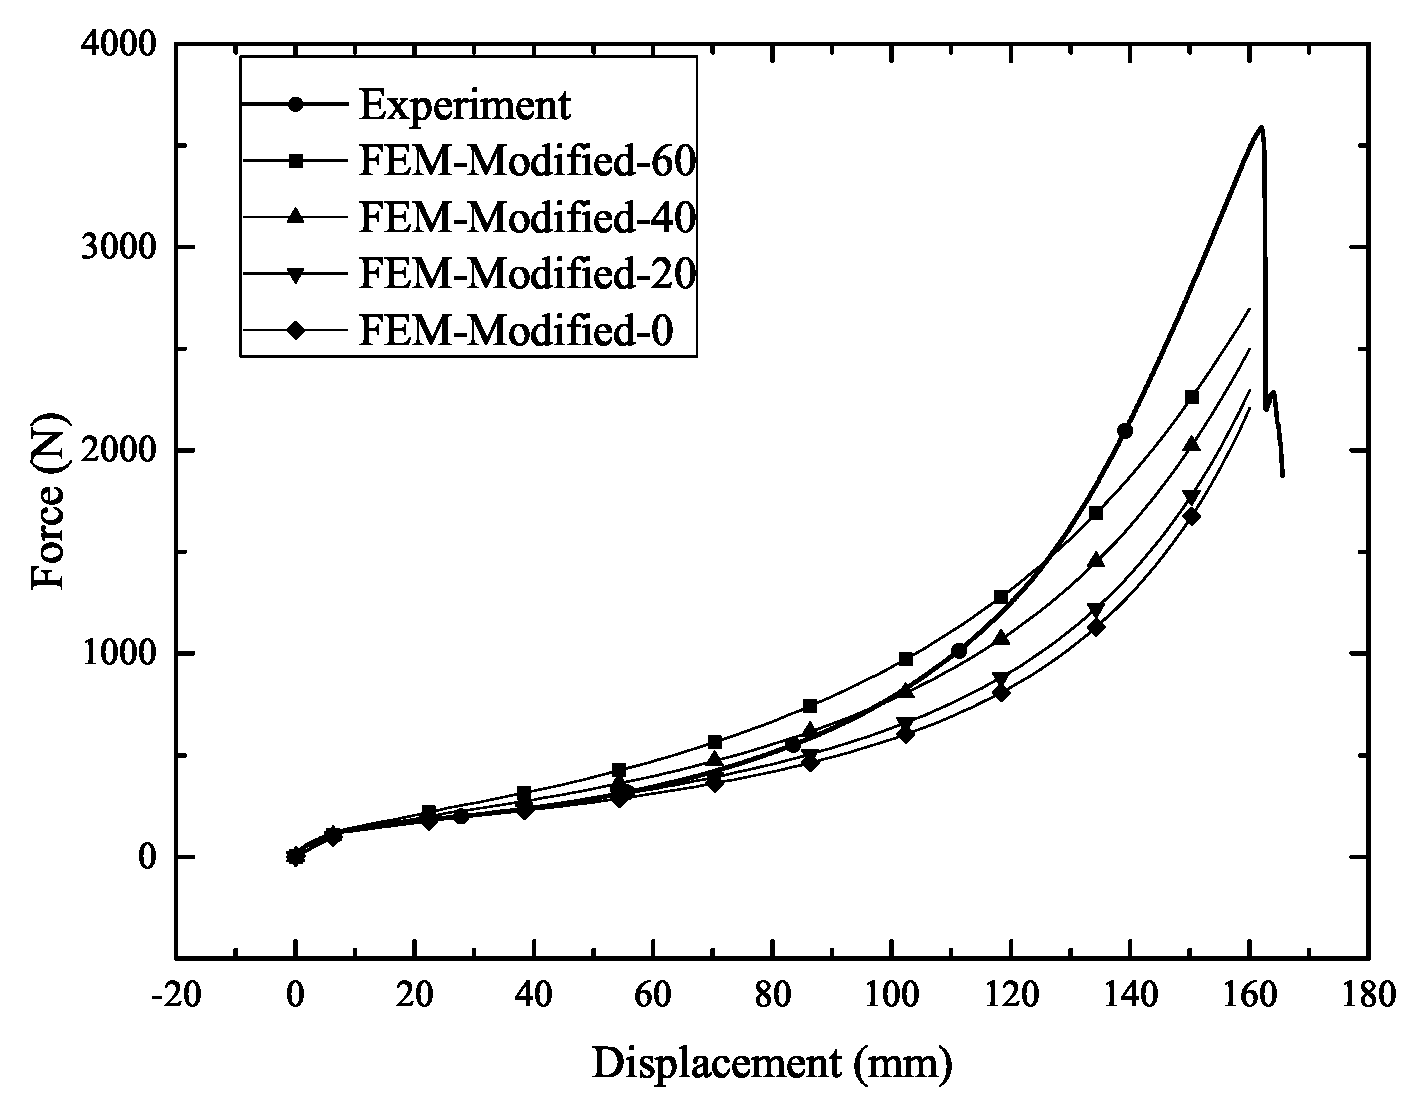
\includegraphics[height=0.35\textheight]{figure/chap5/sp2/phi-MOD}
		}
	\fcaption{纤维偏离角度的影响}{influence of interlacing fiber}
	\label{fig:phi-MOD}
\end{figure*}






\subsection{斜穿纤维体积比例对总体刚度的影响}

对于金属编织层,并不像复合材料编织层可以明确,因为金属纤维刚度较大,倾向于保持斜穿的状态。图\ref{fig:Vw-MOD}中为假设斜穿纤维体积分数从0到1的4中情况,$ V_W $为$ 0 $时,所有纤维都在编织层平面内。$ V_W=1.0  $时,所有纤维都是斜穿纤维。如图\ref{fig:Vw-MOD}中所示,斜穿纤维体积比例对总体刚度的影响不如纤维偏离角度的影响大。


\begin{figure*}[!htp]
\centering
\subfigure[实验试件-1]{
	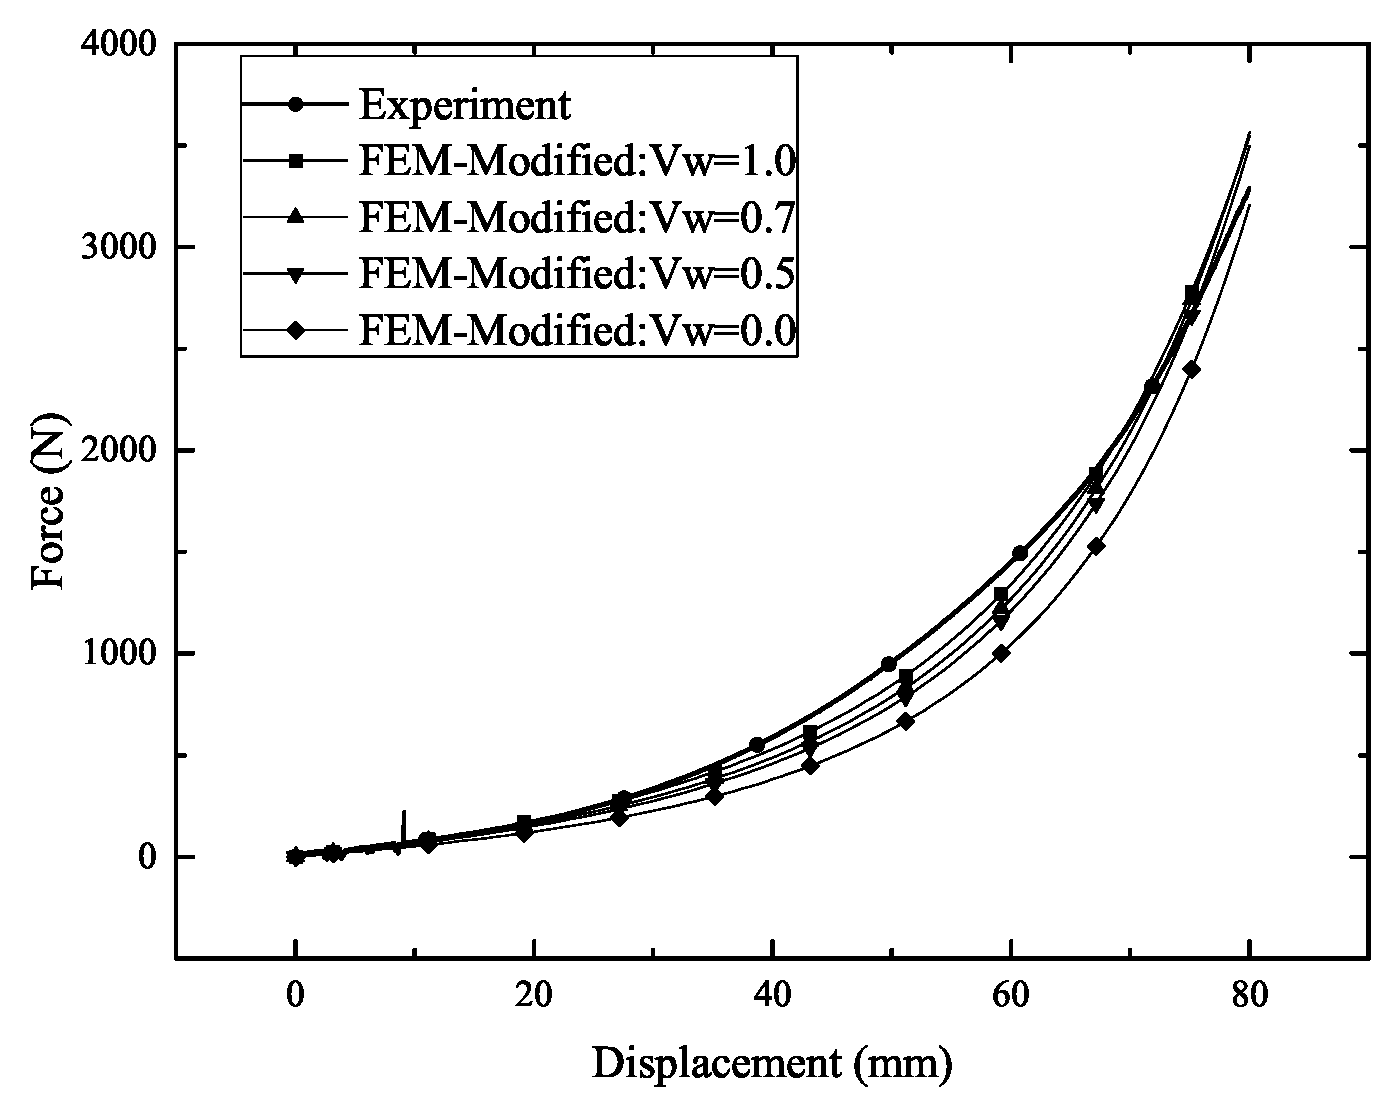
\includegraphics[width=0.7\linewidth]{figure/chap5/sp1/Vw-mod}
	}
\subfigure[实验试件-2]{
	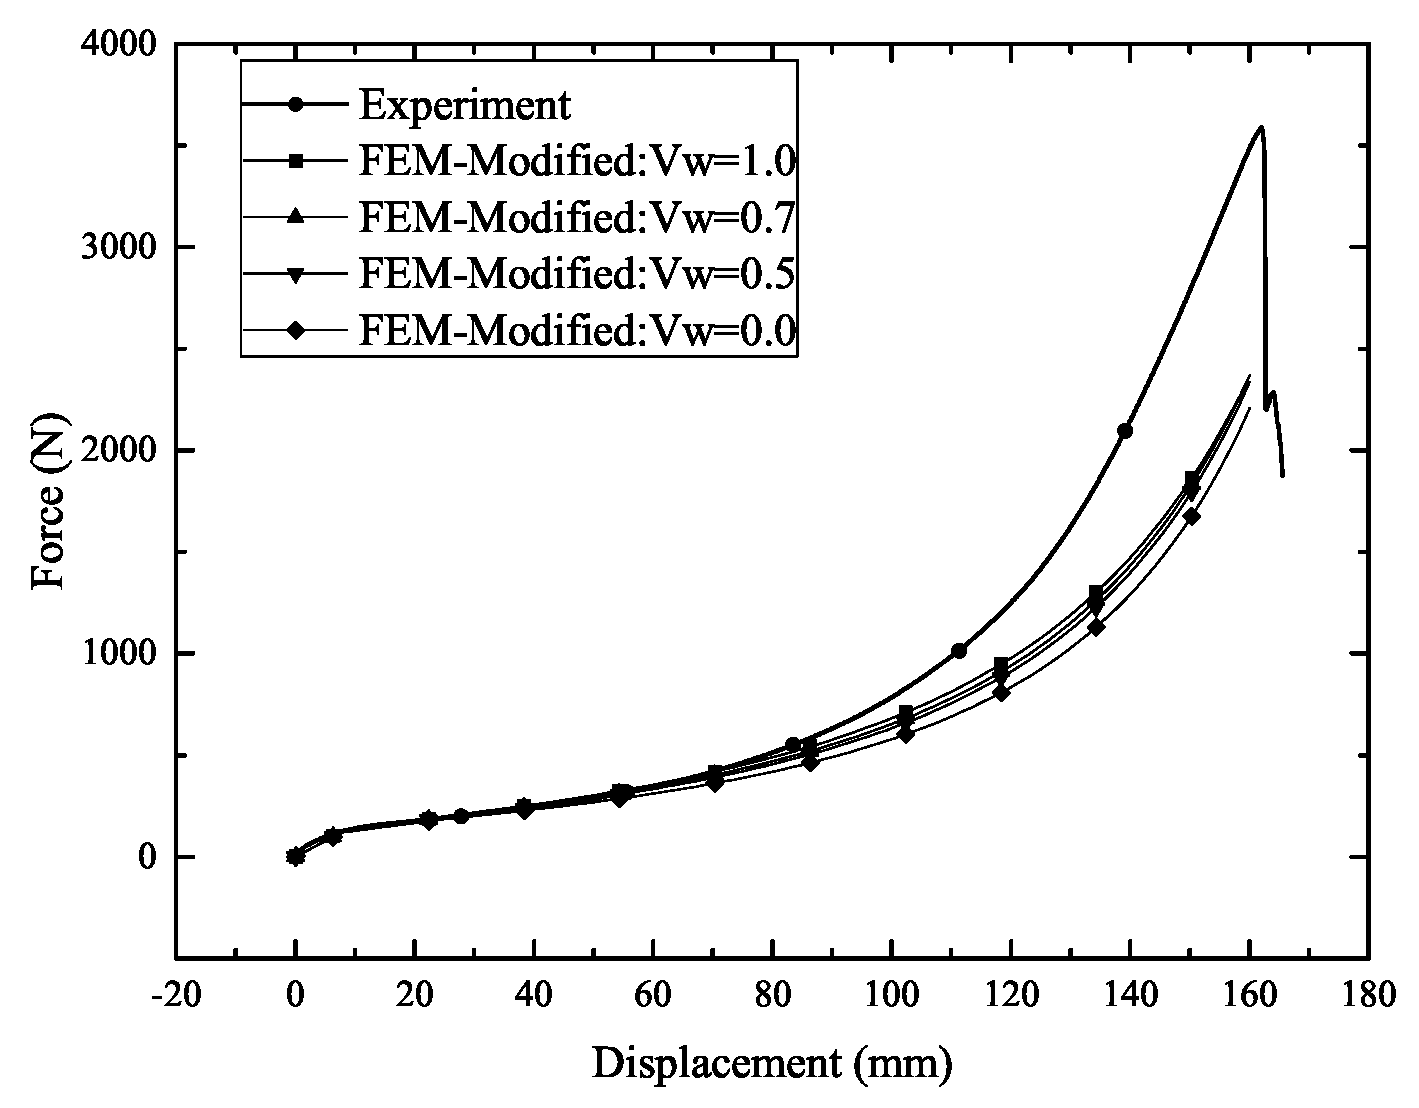
\includegraphics[width=0.7\linewidth]{figure/chap5/sp2/Vw-MOD}
	}
\fcaption{斜穿纤维体积比例对总体刚度的影响}{influence of volume ratio of interlacing fiber}
\label{fig:Vw-MOD}
\end{figure*}






\section{综合修正结果}

考虑以上所有的影响因素的编织层结构非线性行为的影响后,仿真结果的力位移曲线与实验结果仍有一定差距,这部分的差距可以通过编织角加速系数进行修正。如图\ref{fig:k-MOD}所示,基本可以确定$ k\in\left[ 1.10,1.15\right]  $





\begin{figure*}[!htp]
\centering
\subfigure[实验试件-1]{
	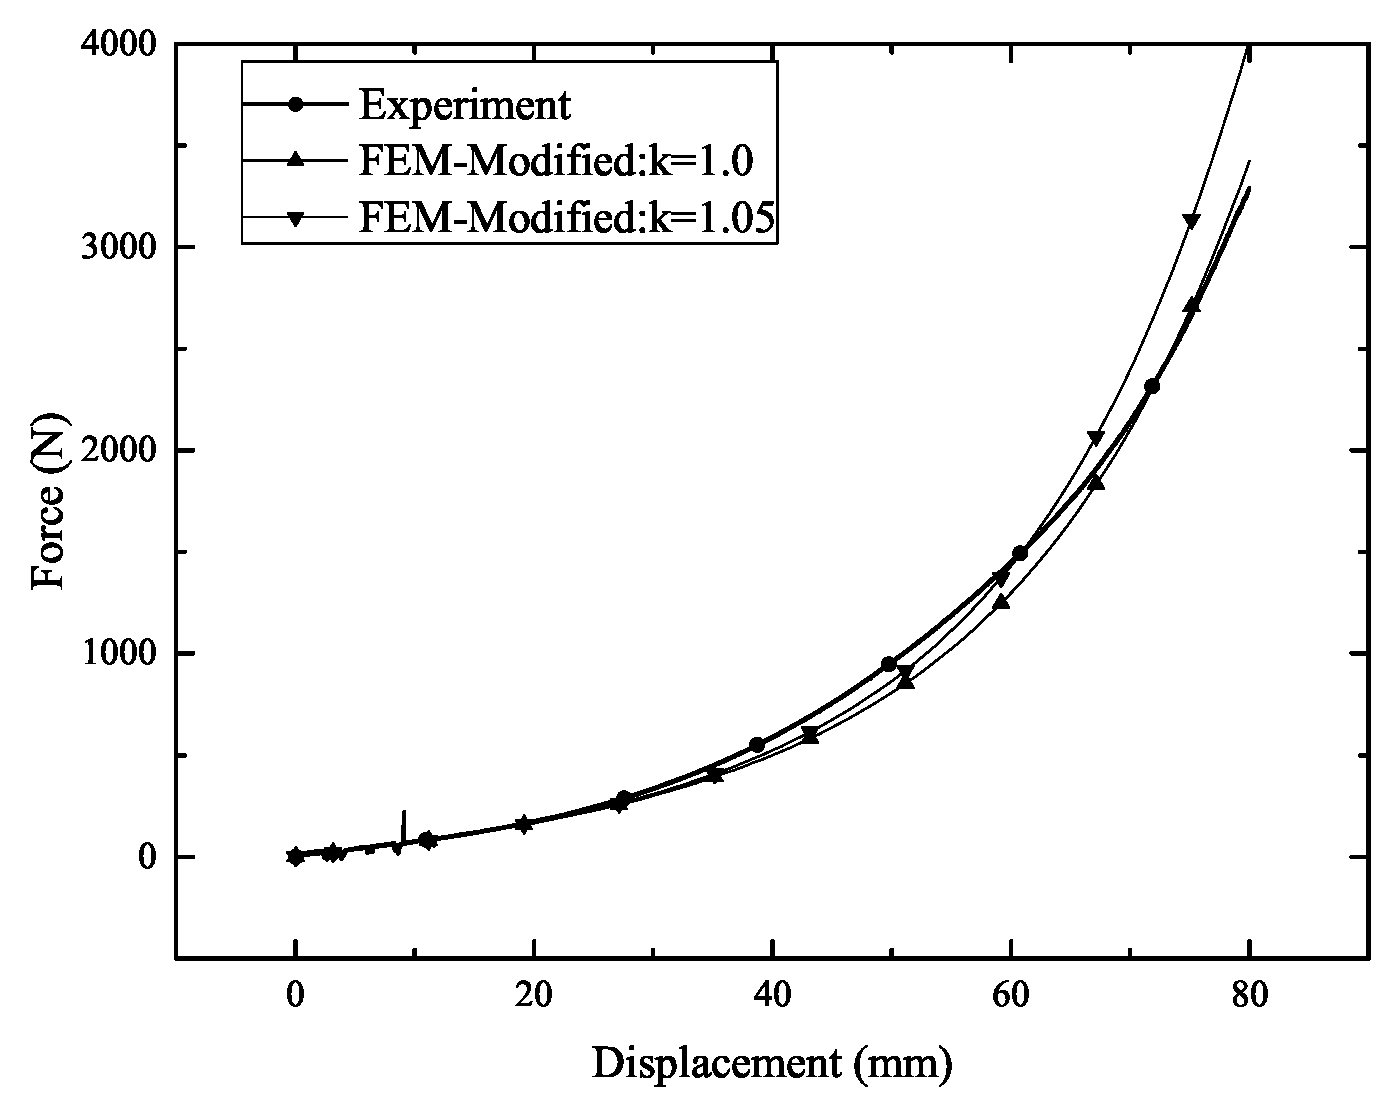
\includegraphics[width=0.7\linewidth]{figure/chap5/sp1/k-mod}
	}
\subfigure[实验试件-2]{
	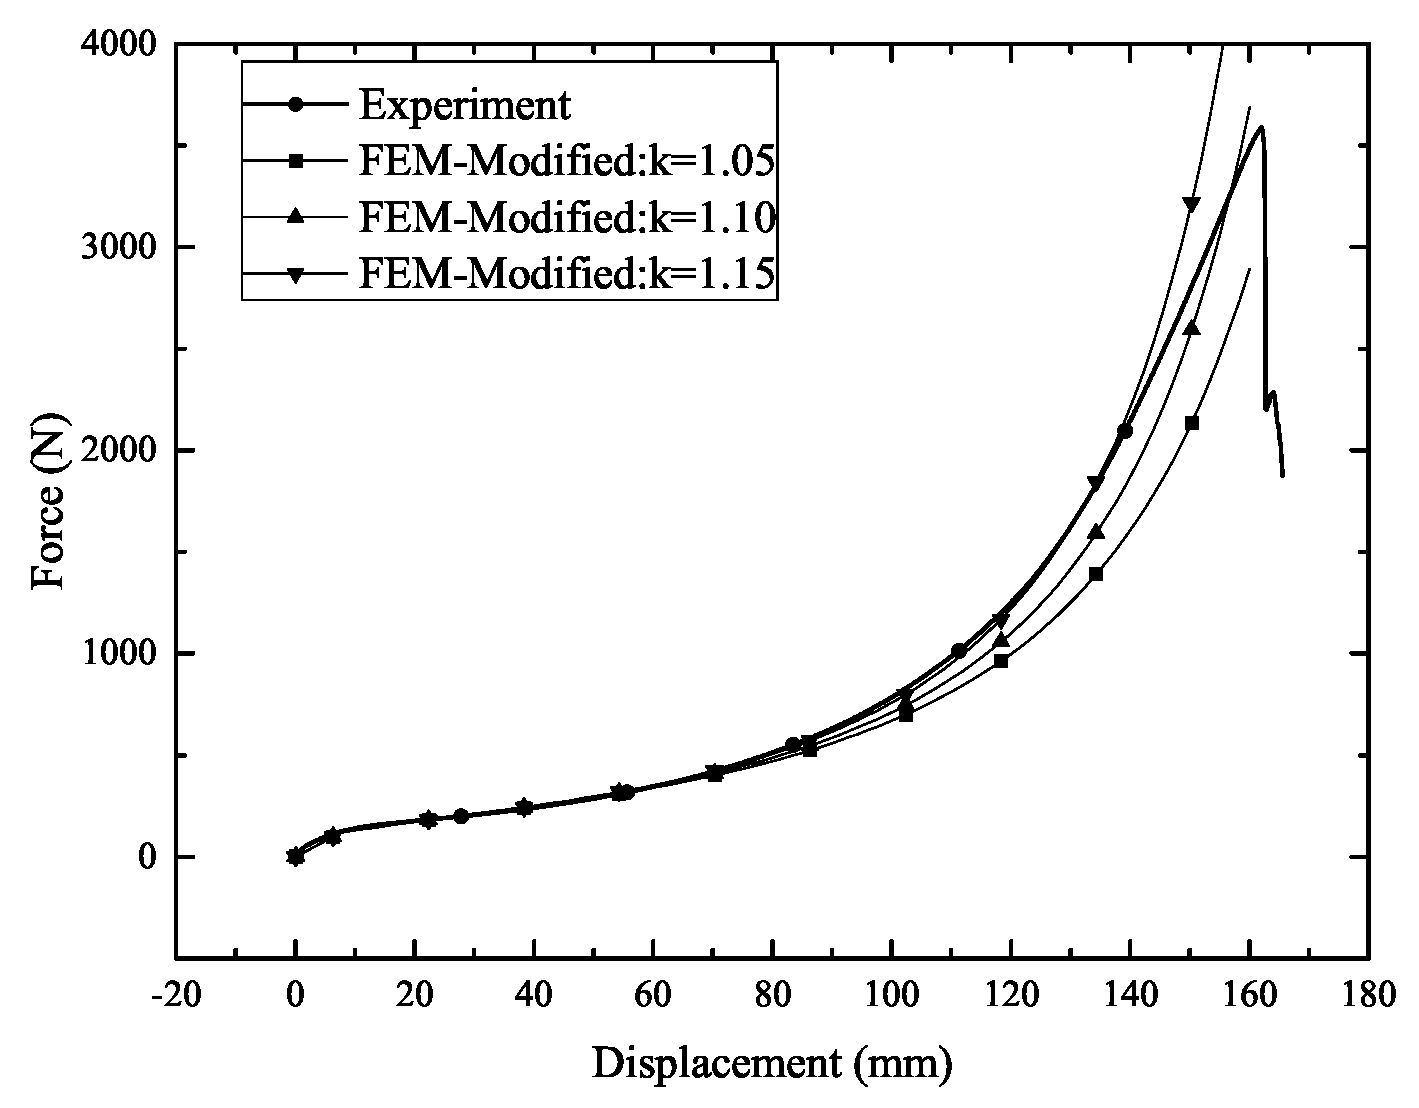
\includegraphics[width=0.7\linewidth]{figure/chap5/sp2/k-MOD}
	}
\fcaption{不同编织角加速系数的影响}{influence of braid angle coefficient}
\label{fig:k-MOD}
\end{figure*}

综合调整其他参数,实验试件-1取$ V_W=1.0$,$ k=1 $;实验试件-2取$ V_W=0.7 $,$ k=1.12 $,仿真结果如\ref{fig:final}所示。

相比 未修正的\ha 基本理论,综合各项影响因素的修正理论基本上可以完全拟合拉伸实验所得到的力位移曲线。所得到的本构理论,从刚度上来说是可信的。从有限元仿真的角度来说,可以较简便地应用于内压爆破实验的仿真。 

\begin{figure*}[!htbp]
\centering
\subfigure[实验试件-1]{
	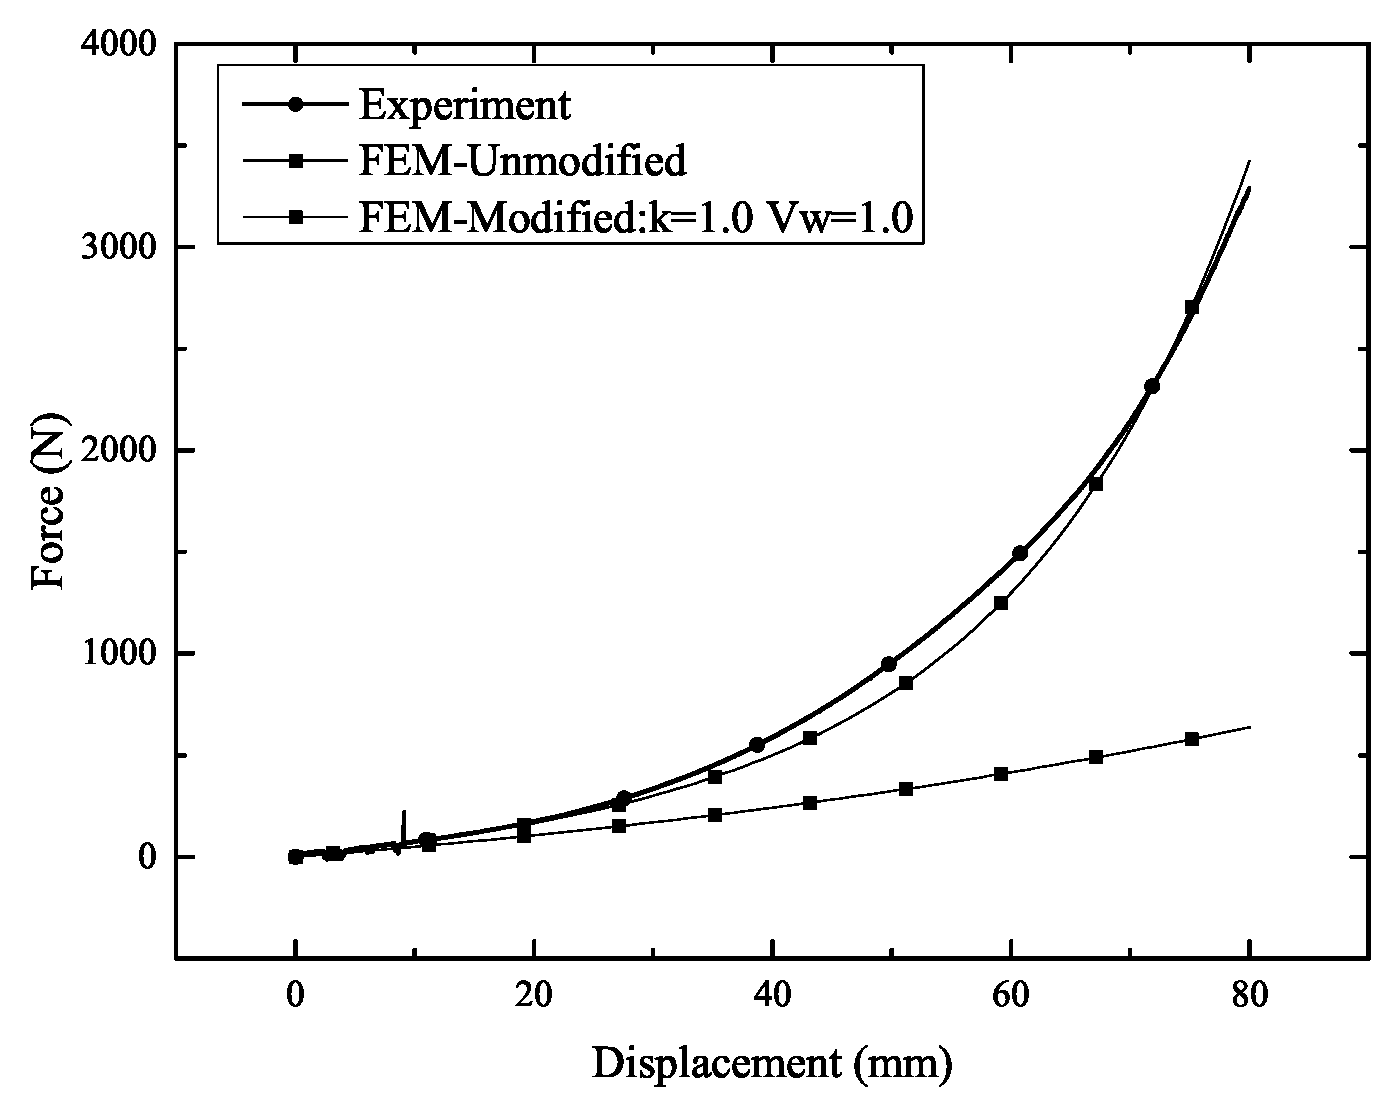
\includegraphics[width=0.7\linewidth]{figure/chap5/sp1/final}
;}
\subfigure[实验试件-2]{
	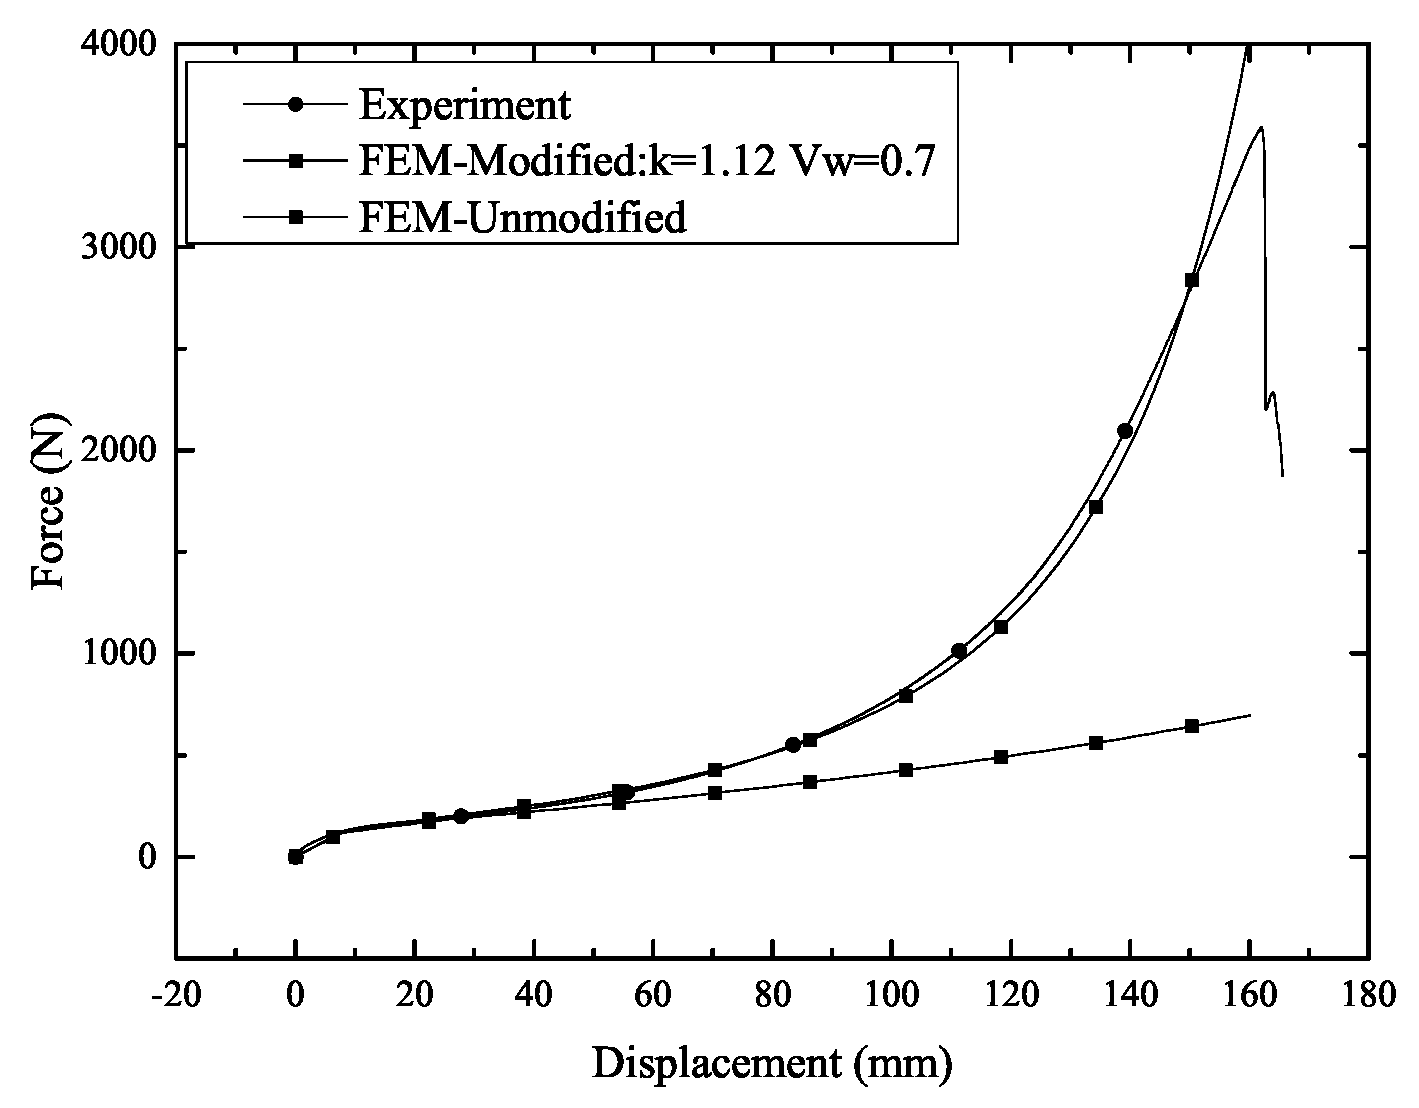
\includegraphics[width=0.7\linewidth]{figure/chap5/sp2/final}
}
\fcaption{综合修正有限元仿真结果}{FEM Results of Modified Model}
\label{fig:final}
\end{figure*}


\section{小 ~ 结}
本章的工作是本研究的重点核心内容,结合拉伸实验获得的实验数据,在\ha 理论的框架体系之上,进行了大量的修正。修正内容包括:
\begin{compactitem}
	\item 利用修正基体法的思路,平均化地引入了纤维间的接触关系,使得总体刚度矩阵满足$ 6\times6 $可以进行三维的有限元分析。
	\item 引入了编织角加速系数,充分反映了编织角的变化,修正了相对实验编织角变化较小的情况,也分析了该系数的物理意义,反映了各股纤维间复杂的传力关系;
	\item 修真特征单元编织角变化的几何关系,将钢绞线理论直接融合到特征单元中,从而使得模型能更好的反应拉伸时,软管管径的变化;
	\item  考虑了纤维在编织层中空间上的分布,区别了斜穿纤维与平面内纤维对整体刚度的贡献;
\end{compactitem}

对理论的修正取得很好的拟合结果,而拟合拉伸实验的意义在于:明确编织层的本构模型,使得模型能够准确的反应拉伸实验中的力学行为。然后将该模型应用于其他工况的仿真。
